\section{Results}

\subsection{Data analysis pipeline}

The initial steps in CoSMoS data analysis involve preprocessing the data set (\FIG{cosmos_experiment}B) to map the spatial relationship between target and binder images, correct for microscope drift (if any) and list the locations of target molecules. Software packages that perform these preprocessing steps are widely available (e.g., \cite{Friedman2015-nx, Smith2019-yb}).

The input into Tapqir consists of the time sequence of images (\FIG{cosmos_experiment}B, right). For colocalization analysis, it is sufficient to consider the image area local to the target molecule. This analyzed area of interest (AOI) needs to be several times the diameter of a diffraction-limited spot to include both the spot and the surrounding background (\FIG{cosmos_experiment}C). 

In addition to AOIs centered at target molecules, it is useful to also select negative control AOIs from randomly selected sites at which no target molecule is present (\FIG{cosmos_experiment}B,D). In Tapqir, such off-target control data is analyzed jointly with on-target data and serves to estimate the background level of target-nonspecific binding. 

Once provided with the preprocessing data and image sequence, Tapqir computes for each frame of each AOI the  probability, $p(\mathsf{specific})$, that a target-specific fluorescence spot is present.   The $p(\mathsf{specific})$ values that are output can then be used to extract information about the kinetics and thermodynamics of the target-binder interaction.

\subsection{Bayesian image classification analysis}

Tapqir calculates $p(\mathsf{specific})$ values using an objective image classification method built on a rigorous Bayesian statistical approach to the CoSMoS image analysis problem. The Bayesian approach has three components. First, we define a probabilistic model of the CoSMoS images. The probabilistic model, \emph{cosmos}, is a mathematical formalism that describes the AOI images in terms of a set of parameter values.  The model is probabilistic in that each parameter is specified to have a probability distribution that defines the likelihood that it can take on particular values. Model parameters describe physically realistic image features such as the characteristic fluorescence spot width. Second, we specify prior distributions for the parameters of the model. These priors embed pre-existing knowledge about the CoSMoS experiment, such as the fact that target-specific spots will be close to the target molecule locations. Third, we infer the values of the model parameters, including $p(\mathsf{specific})$, using Bayes' rule \citep{Bishop2006-oa,Kinz-Thompson2021-tb}. The \emph{cosmos} model is “time-independent”, meaning that we ignore the time dimension of the recording -- the order of the images does not affect the results. 

\subsection{Probabilistic image model and parameters} % Figure 2A,B,C

A single AOI image from a CoSMoS data set is a matrix of noisy pixel intensity values.  In each image, multiple binder molecule fluorescence spots can be present. \FIG{graphical_model}A shows an example image where two spots are present; one spot is located near the target molecule at the center of the image and another is off-target.

The probabilistic model mathematically generates images $D$ as follows.  We construct a noise-free AOI image $\mu^I$ as a constant average background intensity $b$ summed with fluorescence spots modeled as 2-D Gaussians $\mu^S$, which accurately approximate the microscope point spread function \citep{Zhang2007-rb} (\FIG{graphical_model}B). Each 2-D Gaussian is described by parameters integrated intensity $h$, width $w$, and position ($x$, $y$). We define $K$ as the maximum number of spots that can be present in a single AOI image.  For the data we typically encounter, $K$ = 2 is sufficient. Since the spots may be present or not in a particular image, we define the $K$ = 2 binary indicators $m_{\mathsf{spot}(1)}$ and $m_{\mathsf{spot}(2)}$.  Each indicator can take a value of either 0 denoting spot absence or 1 denoting spot presence. 

The resulting mixture model has four possible combinations for $m_{\mathsf{spot}(1)}$ and $m_{\mathsf{spot}(2)}$: (1) a no-spot image that contains only background (\FIG{graphical_model}B, top left), (2) a single-spot image that contains the first binder molecule spot superimposed on background (\FIG{graphical_model}B, bottom left), (3) a single-spot image that contains the second binder molecule spot superimposed on background (\FIG{graphical_model}B, top right), and (4) a two-spot image that contains both binder molecule spots superimposed on background (\FIG{graphical_model}B, bottom right).

Among the spots that are present in an AOI image, by assumption at most only one can be target-specific. We use a \emph{state} parameter $z$ to indicate target-specific spot absence ($z=0$) or presence ($z=1$) in an AOI image. We also introduce an \emph{index} parameter $\theta$ that identifies which of the spots is the target-specific spot  when it is present ($z = 1$) (e.g., \FIG{graphical_model}C, middle and right have $\theta = 1$ and $\theta = 2$, respectively) and equals zero when it is absent ($z = 0$) (e.g., \FIG{graphical_model}C, left). Since the off-target control AOIs by definition contain only non-specific binding, $z = 0$ and $\theta = 0$ for all off-target AOIs. 

Finally, to construct realistic noisy AOI images $D$ from the noise-free images $\mu^I$, the model adds intensity-dependent noise to each pixel.  Each measured pixel intensity in a single-molecule fluorescence image has a noise contribution from photon counting (shot noise) and can also contain additional noise arising from electronic amplification \citep{Van_Vliet1998-jk}. The result is a characteristic linear relationship between the noise variance and mean intensity with slope defining the gain $g$. This relationship is used to compute the random pixel noise values (see Materials and Methods).

The resulting probabilistic image model can be interpreted as a generative process that produces the observed image data $D$. A graphical representation of the probabilistic relationships in the model is shown in \FIG{graphical_model}D. A complete description of the model is given in Materials and Methods and \FIGSUPP[graphical_model]{extended}.  
 
\begin{figure}
\begin{fullwidth}
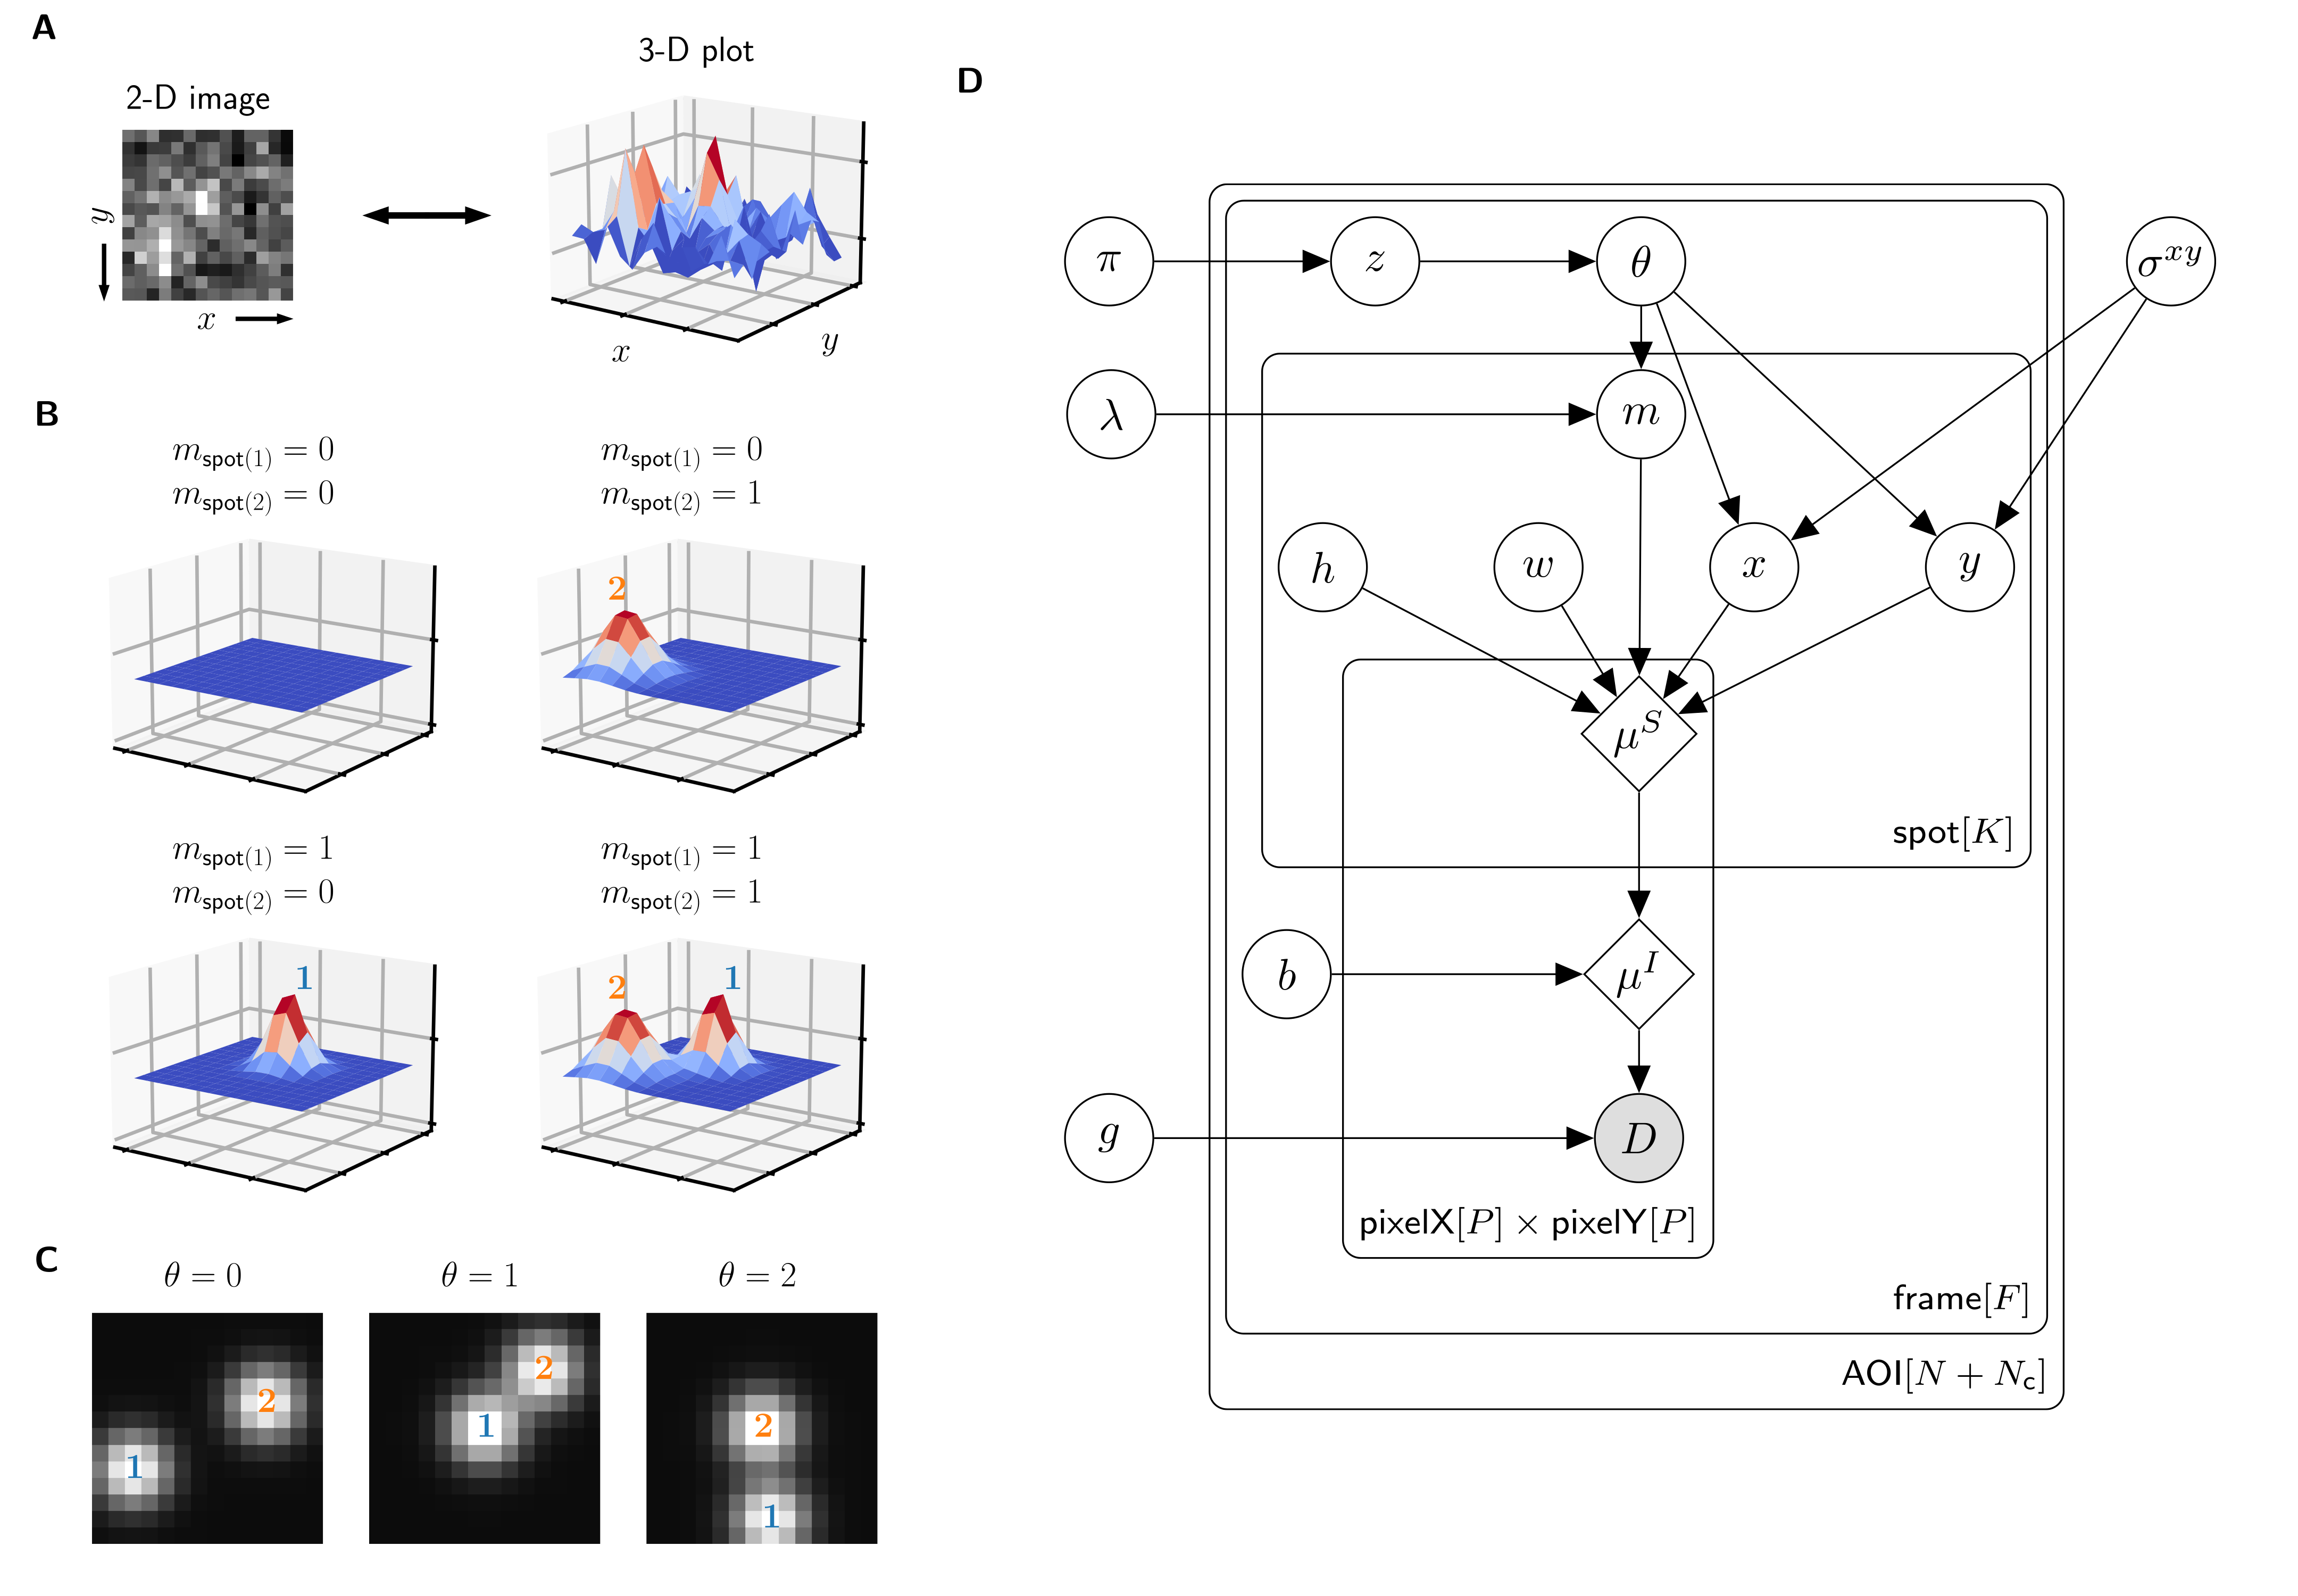
\includegraphics[width=183mm]{figures/graphical_model.png}
\caption{\textbf{Depiction of the probabilistic image model and model parameters.} (\textbf{A}) Example AOI image from the Data set A in \TABLE{datasets}. The AOI image is a matrix of $14 \times 14$ pixel intensities which is shown here as both a 2-D grayscale image and as a 3-D intensity plot. The image contains two spots, one is centered at target location (image center) and the other is located off-target. (\textbf{B}) Examples of four idealized noise-free image representations ($\mu^I$). Image representations consist of zero, one, or two idealized spots ($\mu^S$) superimposed on a constant background ($b$). Each fluorescent spot is represented as a 2-D Gaussian parameterized by integrated intensity ($h$), width ($w$), and position ($x$, $y$). The presence of spots is encoded in the binary spot existence indicator $m$. (\textbf{C}) Simulated idealized images illustrating different values of the target-specific spot index parameter $\theta$. $\theta = 0$ corresponds to a case when no specifically bound molecule is present; $\theta = 1$ or 2 corresponds to the cases in which the specifically bound molecule is spot 1 or 2, respectively. (\textbf{D}) Condensed graphical representation of the probabilistic model. Model parameters are depicted as circles and deterministic functions as diamonds. Observed image ($D$) is represented by a shaded circle. Related nodes are connected by edges, with an arrow pointing towards the dependent node (e.g., the shape of each 2-D Gaussian spot $\mu^S$ depends on spot parameters $m$, $h$, $w$, $x$, and $y$). Plates (rounded rectangles) contain entities that are repeated for the number of instances displayed at the bottom-right corner: number of total AOIs ($N+N_\mathsf{c}$), frame count ($F$), and maximum number of spots in a single image ($K=2$). Parameters outside of the plates are global quantities that apply to all frames of all AOIs. A more complete version of the graphical model specifying the relevant probability distributions is given in \FIGSUPP[graphical_model]{extended}a. }
\label{fig:graphical_model}
\figsupp[Extended graphical representation of the generative probabilistic model and the prior distributions for $x$ and $y$ spot position parameters.]{\textbf{Extended graphical representation of the generative probabilistic model and the prior distributions for $x$ and $y$ spot position parameters.} \textbf{a}, Directed factor graph representation \cite{Bishop2006-oa} of model parameters and parameter distributions. This diagram is a more complete version of the graphical model shown in \FIG{graphical_model}d; it includes additional parameters ($\mu^b$, $\sigma^b$, $\delta$) and explicitly specifies the relevant probability distributions.  Model parameters are depicted as circles, parameter distributions as small filled squares, and deterministic functions as diamonds. Names of the probability distributions are written next to the squares. Input parameters and output parameters are connected by lines, with an arrow pointing towards the dependent parameter. Observed image ($D$) is the sum of the noisy photon-dependent image ($I$) and the photon-independent camera offset ($\delta$). Plates (rounded rectangles) contain nodes that are repeated for the number of instances displayed at the bottom-right corner: number of AOIs ($N+N_\mathsf{c}$), frame count ($F$), maximum number of spots in a single image ($K$), and number of image pixels ($P \times P$). \textbf{b}, Prior distributions of $x$ and $y$ for specific and non-specific binding. Probability densities for $x$ and $y$ are defined in the range $\left[ -(P+1)/2, (P+1)/2 \right] $ relative to the target molecule and are conditional on the identity of the spot (specific or non-specific).  Probability densities for $x$ and $y$ parameters are identical. }{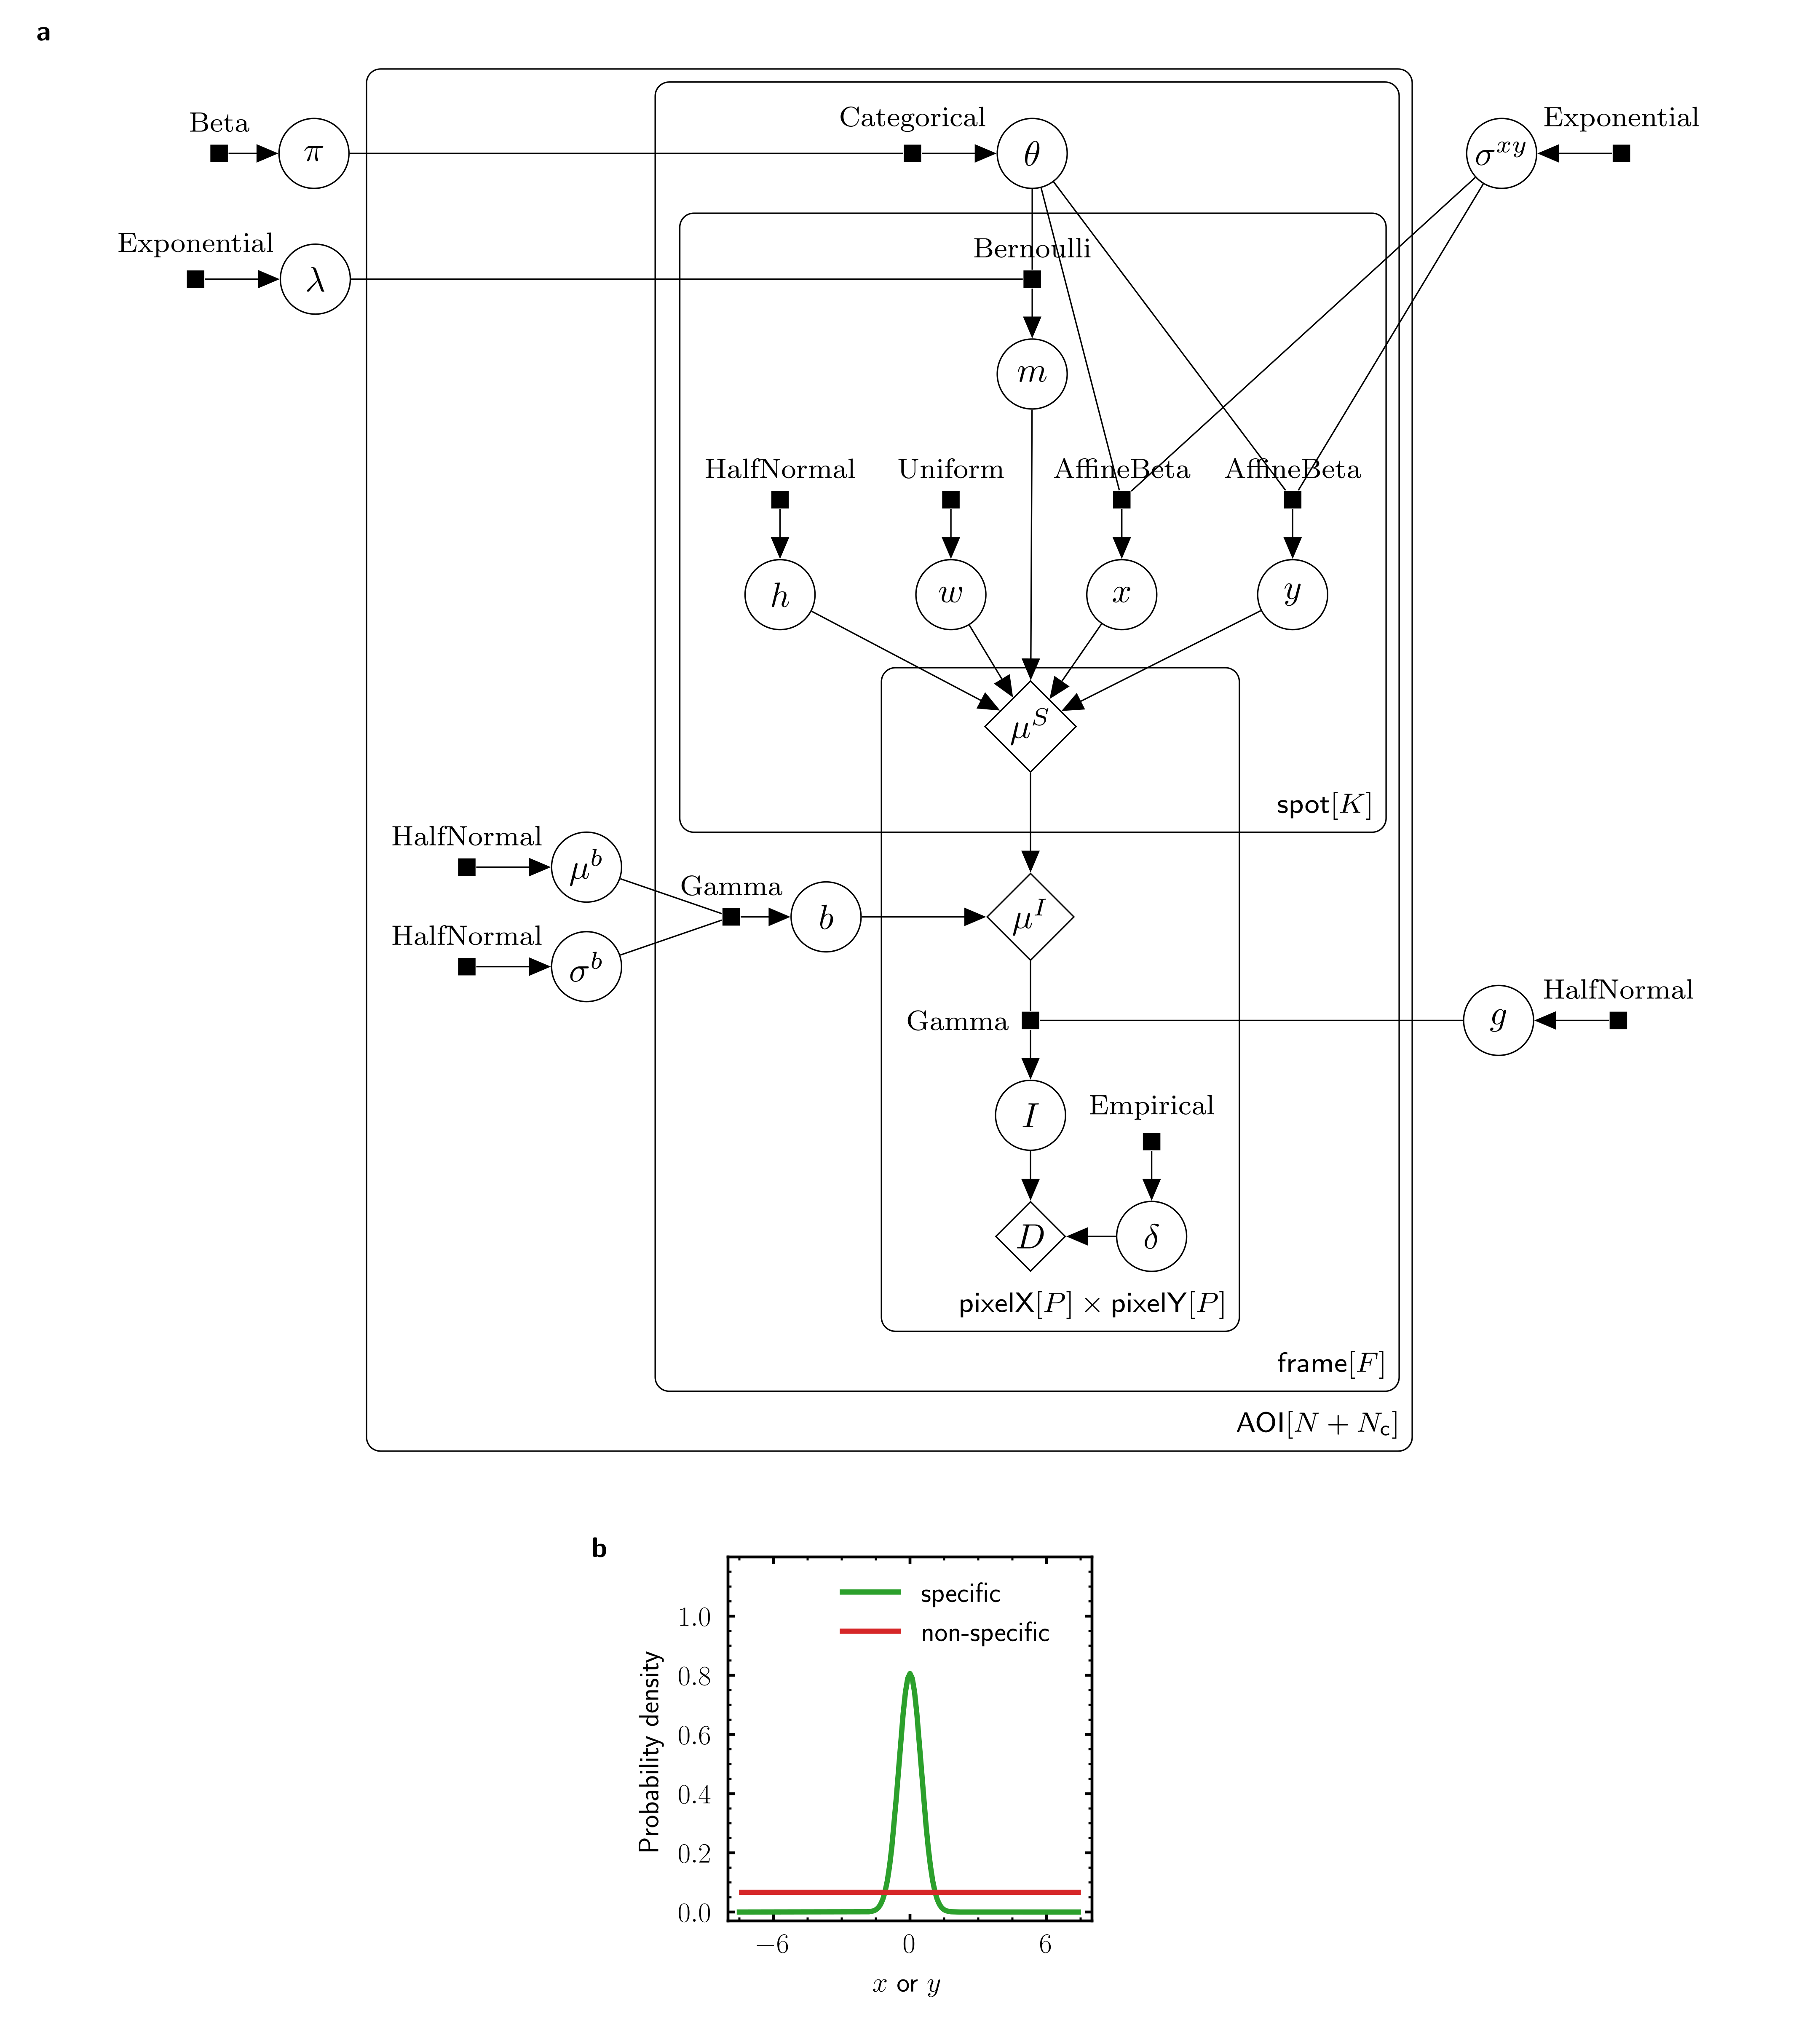
\includegraphics[width=183mm]{extended-data/figure1.png}}\label{figsupp:extended}
\end{fullwidth}
\end{figure}

\subsection{Parameter prior distributions}

Specifying prior probability distributions for model parameters is essential for Bayesian analysis and allows us to incorporate pre-existing knowledge about the experimental design. For most model parameters, there is no strong prior information so we use uninformative prior distributions (see Materials and Methods). However, we have strong expectations for the positions of specific and non-specific binder molecules that can be expressed as prior distributions and used effectively to discriminate between the two. Non-specific binding can occur anywhere on the surface with equal probability and thus has a uniform prior distribution across the AOI image. Target-specific binding, on the other hand, is colocalized with the target molecule and thus has a prior distribution peaked at the AOI center (\FIGSUPP[graphical_model]{xy}). The width of this peak, proximity parameter $\sigma^{xy}$, depends on multiple features of the experiment such as the spot localization accuracy and the mapping accuracy between target and binder imaging channels. Prior distributions for parameters $\theta$ and $m$ are defined in terms of the average number of target-specific and target non-specific spots per AOI image, $\pi$ and $\lambda$, respectively. To facilitate convenient use of the algorithm, it is not necessary to pre-specify values of $\sigma^{xy}$, $\pi$, and $\lambda$.  Instead, values of these parameters appropriate to a given data set are calculated automatically using a hierarchical Bayesian analysis (see Materials and Methods; for hierarchical modeling see Chapter 5 of \cite{Gelman2013-ro}).

\subsection{Bayesian inference and implementation}

Tapqir calculates posterior distributions of model parameters conditioned on the observed data by using Bayes' theorem. In particular, Tapqir approximates posterior distributions using a variational inference approach implemented in Pyro \citep{Bingham2019-qy}.  Complete details of the implementation are given in Materials and Methods.

\subsection{Tapqir analysis}

To test the approach, we used Tapqir to analyze simulated CoSMoS image data with a comparatively high SNR of 3.76 as well as data from the experiment shown in \FIG{cosmos_experiment}B-D, which has a lower SNR of 1.61. The simulated data were generated using the same \emph{cosmos} model (\FIG{graphical_model}D) that was used for analysis. Tapqir correctly detects fluorescent spots in both simulated and experimental images (compare ``AOI images'' and ``Spot-detection'' rows in \FIG{tapqir_analysis}). The program precisely calculates the position ($x$, $y$), intensity ($h$), and width ($w$) for each spot and also determines the background intensity ($b$) for each image without requiring a separate analysis. These parameters confirm the desired behavior of the model and could be used in further calculations.  However, the most important output of the analysis is assessment of the presence of target-specific binding.  For each AOI image, we calculate $p(\mathsf{specific}) \equiv p(z=1)$ (\FIG{tapqir_analysis}, green), the probability that any target-specific spot is present. Spots determined as likely target-specific ($p(\mathsf{specific}) > 0.5$) are represented as filled circles in the spot detection row of \FIG{tapqir_analysis}. For a particular spot to have high $p(\mathsf{specific})$, it must have a high spot probability and be colocalized with the target molecule at the center of the AOI (\FIGSUPP[tapqir_analysis]{probs}).  

\begin{figure}
\begin{fullwidth}
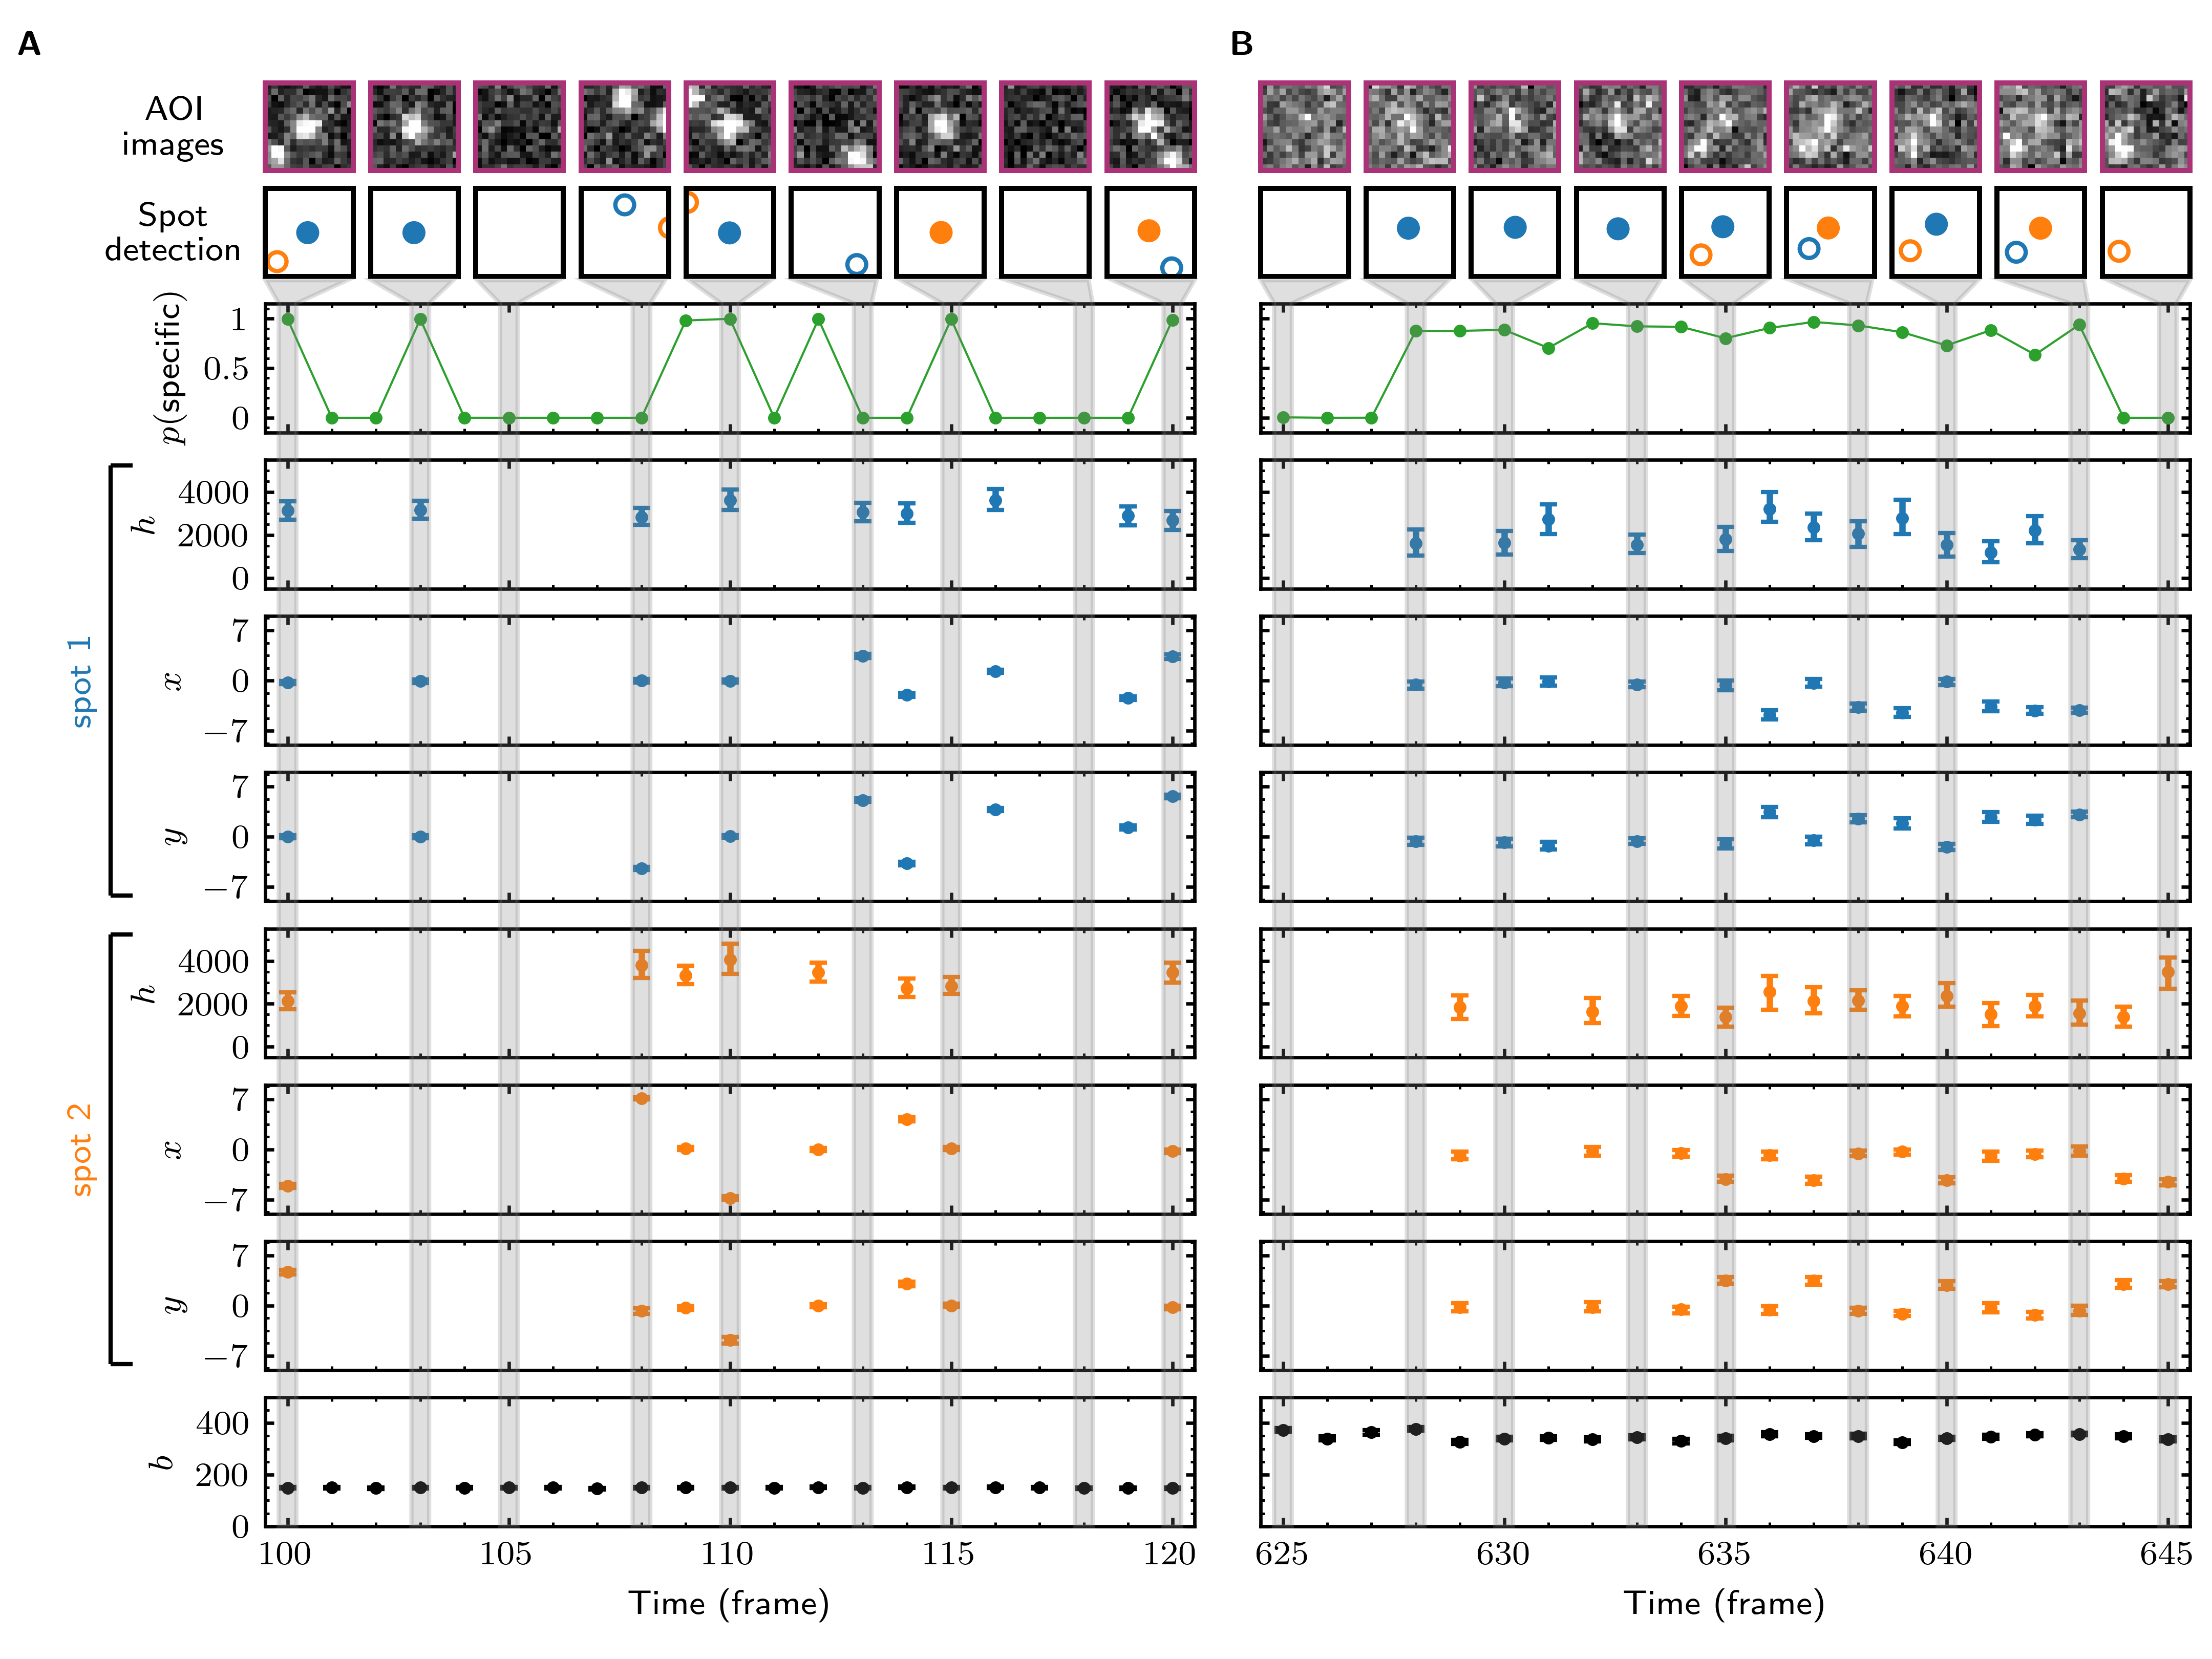
\includegraphics[width=183mm]{figures/tapqir_analysis.png}
\caption{\textbf{Tapqir analysis and inferred model parameters.} (\textbf{A},\textbf{B}) Tapqir was applied to simulated data (\texttt{lamda0.5} parameter set in Supplemental Data 1) (\textbf{A}) and to experimental data (Data set A in \TABLE{datasets}) (\textbf{B}). (\textbf{A}) and (\textbf{B}) each show a short extract from a single target location in the data set. The first row shows AOI images for the subset of frames indicated by gray shaded stripes in the plots; image contrast and offset settings are consistent within each panel. The second row shows the locations of spots determined by Tapqir. Spot numbers 1 (blue) and 2 (orange) are assigned arbitrarily and may change from fame to frame. For clarity, only data for spots with a spot probability $p(m=1) > 0.5$ are shown. Spots predicted to be target-specific ($p(\theta=k)>0.5$ for spot $k$) are shown as filled circles. The topmost graphs (green) show the calculated probability that a target-specific spot is present ($p(\mathsf{specific})$) in each frame.  Below are the calculated spot intensities ($h$), spot widths ($w$), and locations ($x$, $y$) for spot 1 (blue) and spot 2 (orange), and the AOI background intensities ($b$).  Again, for clarity data are only shown for likely spots ($p(m=1) > 0.5$). Error bars: 95\% CI (credible interval) estimated from a sample size of 500.  Some error bars are smaller than the points and thus not visible.}
\label{fig:tapqir_analysis}

\figsupp[Calculated spot probabilities.]{\textbf{Calculated spot probabilities. } The data sets used for panels A and B are identical to those in  \FIG{tapqir_analysis} A and B; the first two rows and the  $p(\mathsf{specific})$ (green) graph are reproduced from that figure. Blue graphs show the probability of being present ($p(m=1)$) and of being target-specific ($p(\theta=1)$) for the arbitrarily designated spot 1 in each frame.  Orange graphs show the analogous quantities $p(m=1)$ and $p(\theta=2)$ for spot 2. For a given image, the probability $p(\mathsf{specific}) \equiv p(z=1)$ that any target-specific spot is present is equal to $p(\theta=1) + p(\theta=2)$.}{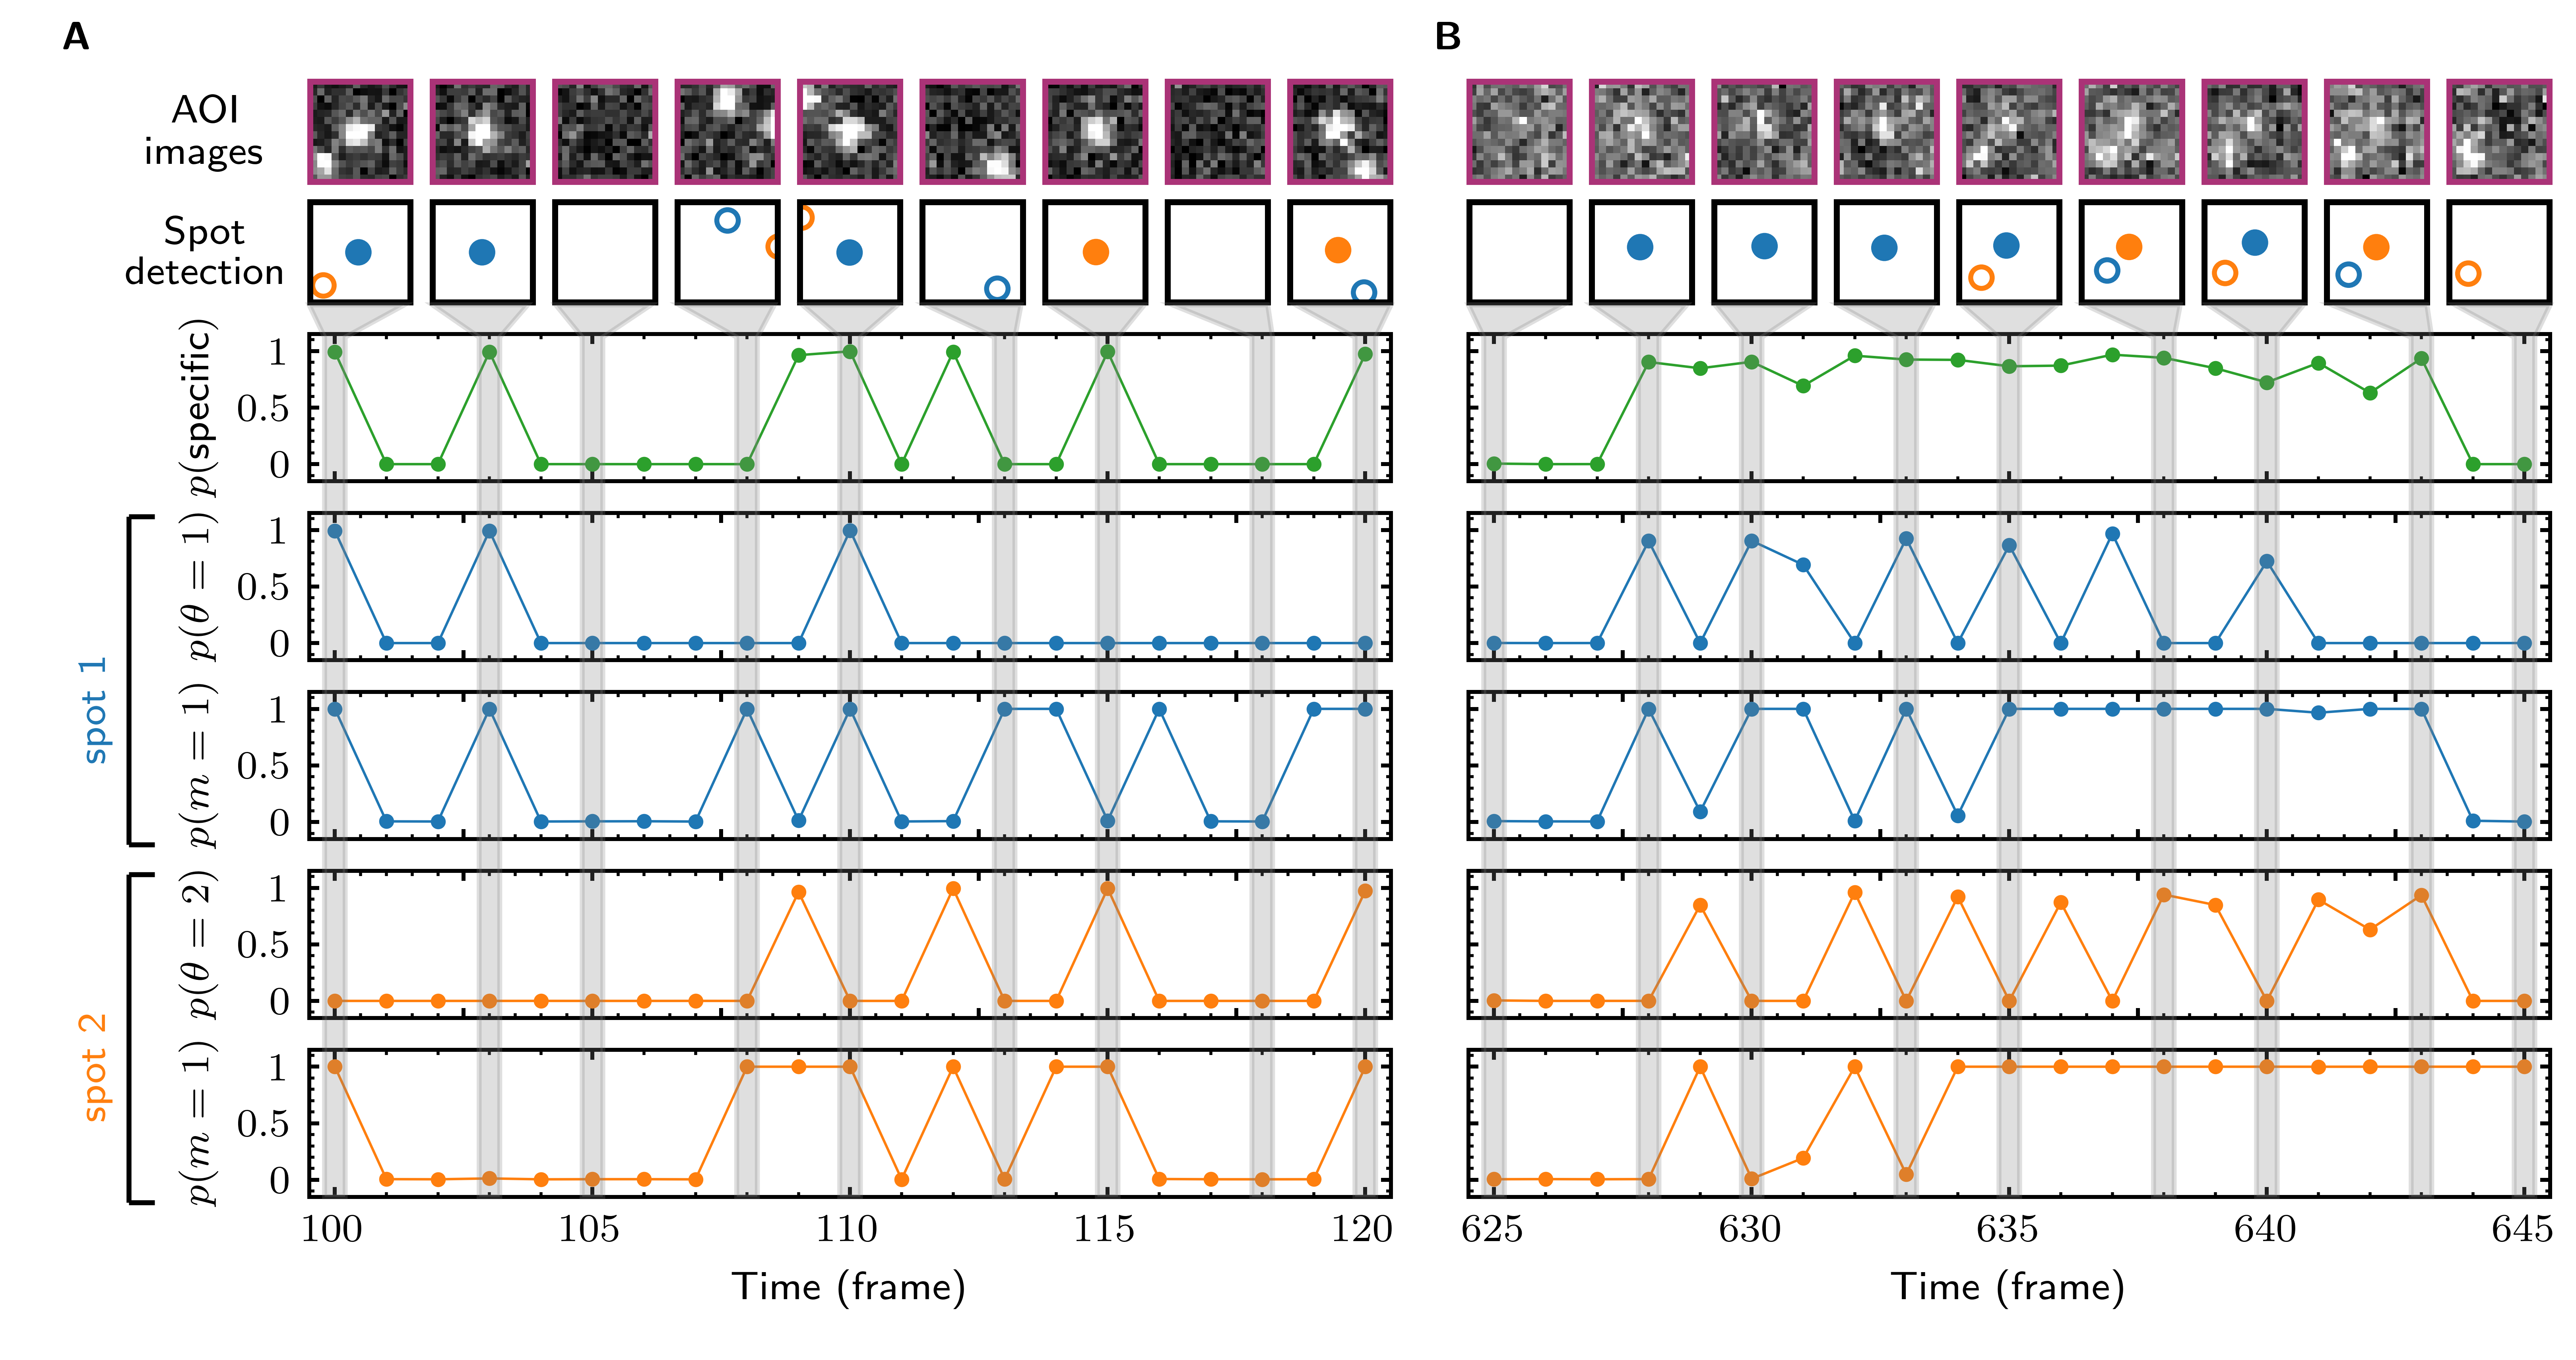
\includegraphics[width=183mm]{figures/tapqir_analysis_probs.png}}\label{figsupp:probs}

\figsupp[Reproduction of experimental data by posterior predictive sampling.]{\textbf{Reproduction of experimental data by posterior predictive sampling.} Example frames are shown from Data set A  (\textbf{A}: SNR = 1.61), Data set B (\textbf{B}: SNR = 3.77), Data set C (\textbf{C}: SNR = 4.23), and Data set D (\textbf{D}: SNR = 3.06) in \TABLE{datasets}. In each panel the top row shows AOI images selected from the experimental data and middle row shows corresponding images obtained by sampling from the posterior distributions. Image contrast and offset are consistent within each panel. The bottom row shows pixel intensity distributions from the experimental and posterior prediction images.}{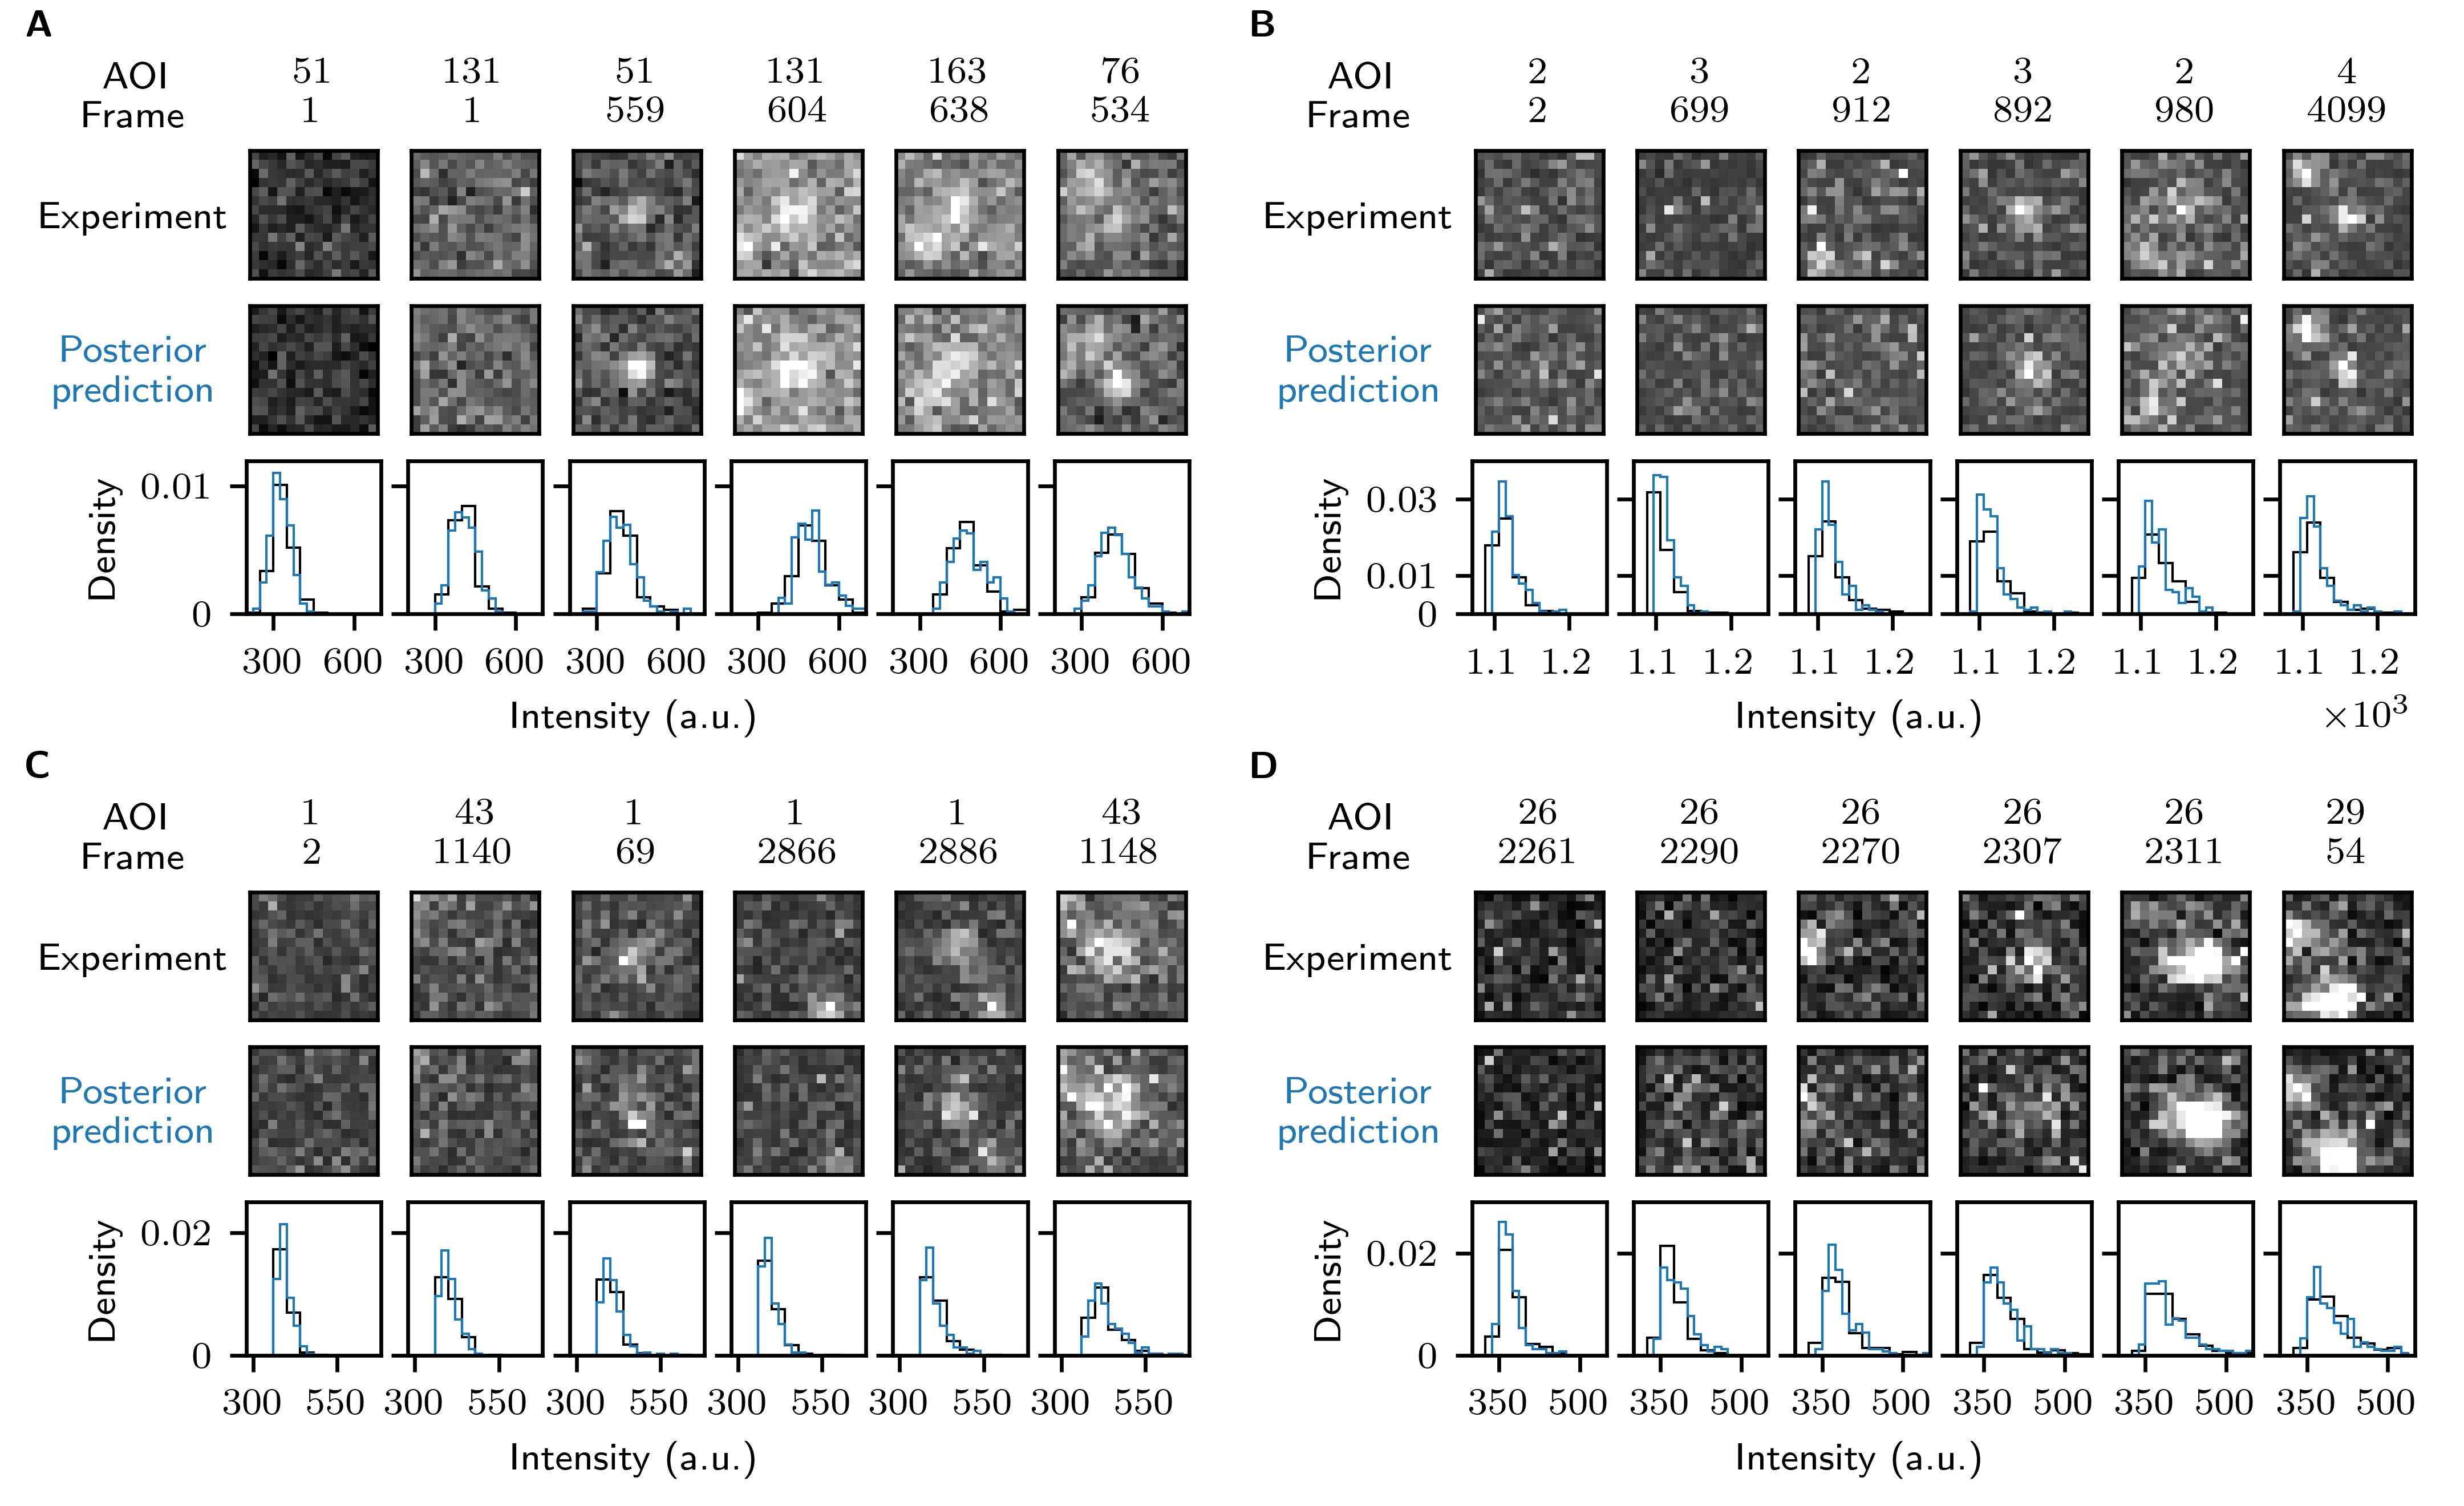
\includegraphics[width=183mm]{figures/tapqir_analysis_ppc.png}}\label{figsupp:ppc}

\figsupp[Tapqir analysis of image data simulated using a broad range of global parameters.]{\textbf{Tapqir analysis of image data simulated using a broad range of global parameters.} Simulations (see Materials and Methods) consist of 16 data sets where values of global parameters ($\pi$, $\lambda$, $\sigma^{xy}$, and $g$) where randomly generated for each data set (Supplemental Data 2). Simulated data were fit with Tapqir, and parameter values from the fit (with 95\% credible interval estimated from a sample size of 10,000) are plotted against the true parameter values. To guide the eye, dashed lines  indicate identical true and fit values. (\textbf{A}) Gain of the camera $g$. (\textbf{B}) Average target-specific binding probability $\pi$. (\textbf{C}) Target non-specific binding density $\lambda$. (\textbf{D}) Proximity parameter $\sigma^{xy}$.}{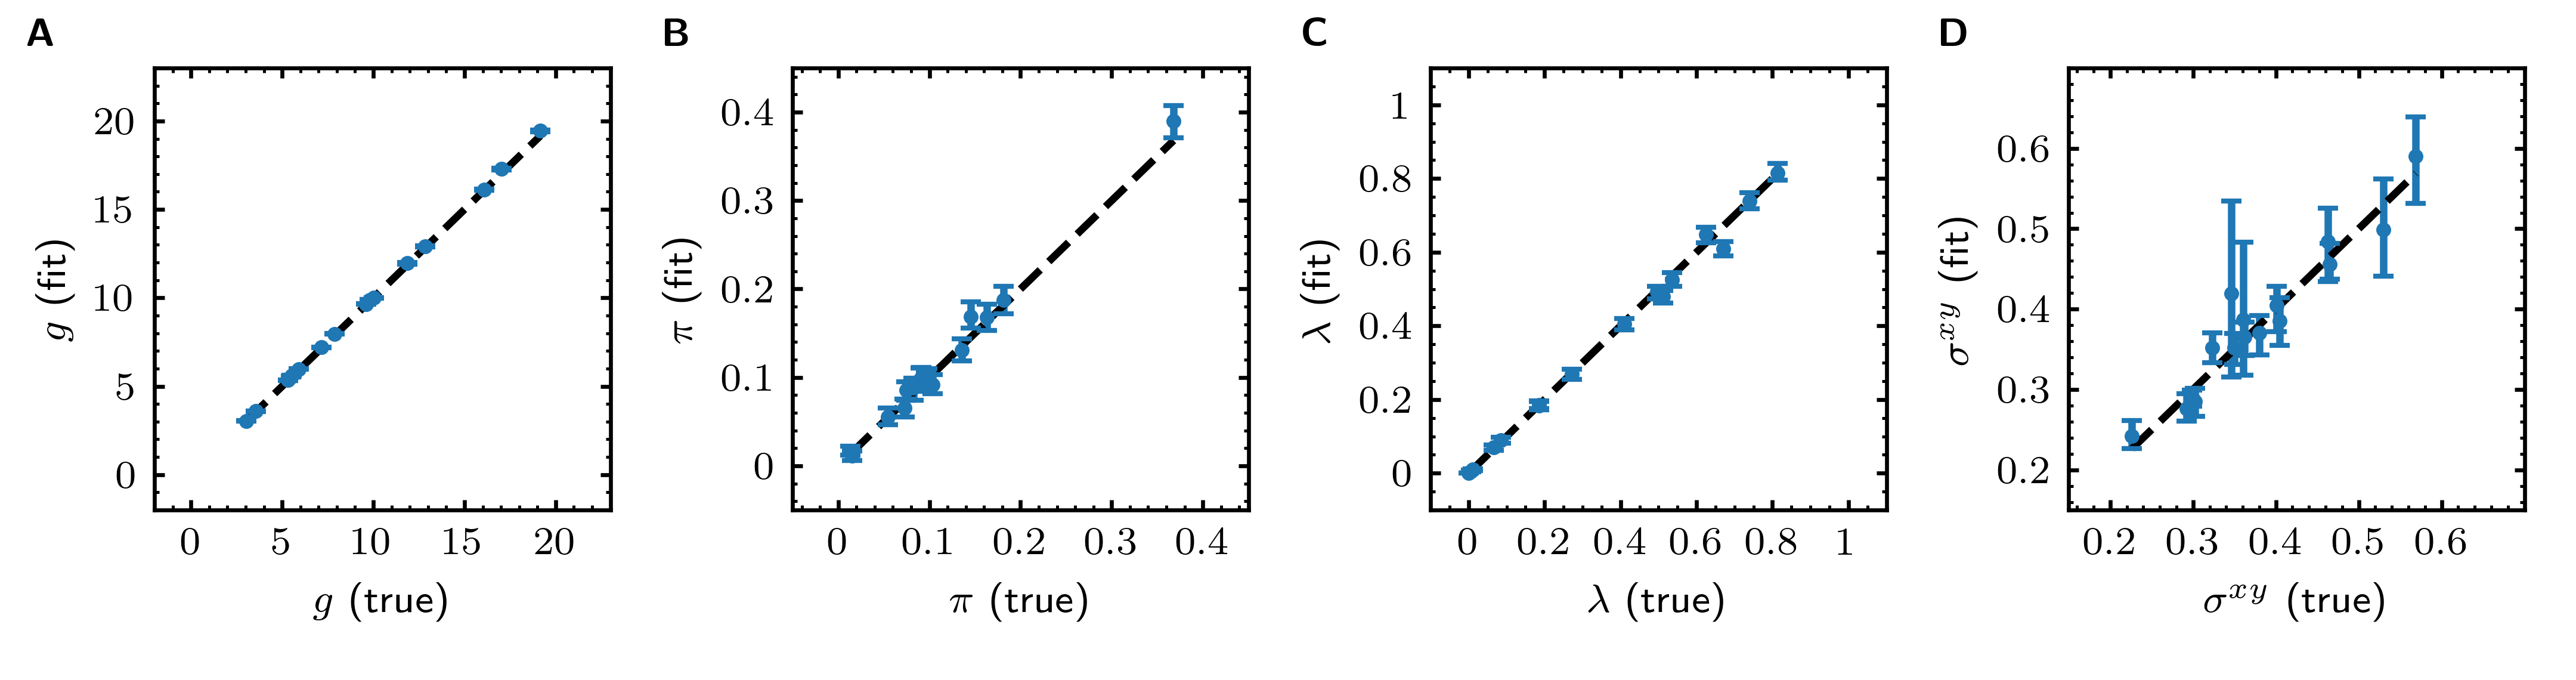
\includegraphics[width=183mm]{figures/tapqir_analysis_randomized.png}}\label{figsupp:randomized}

\figsupp[Effect of AOI size on analysis of experimental data.]{\textbf{Effect of AOI size on analysis of experimental data.} (\textbf{A}) and (\textbf{B}) each show a short extract from a single target location (AOI 163 in (\textbf{A}) and AOI 0 in (\textbf{B})) from Data set A (\TABLE{datasets}; SNR = 1.61). Tapqir was applied to the data set using AOI image sizes $P$ of $14 \times 14$ (first row), $10 \times 10$ (second row), and $6 \times 6$ (third row) pixels. Corresponding output $p(\mathsf{specific})$ probabilities are plotted in the graph. Image contrasts in (\textbf{A}) and (\textbf{B}) are different. Unattended calculation time on an AMD Ryzen Threadripper 2990WX with an Nvidia GeForce RTX 2080Ti GPU using CUDA version 11.5 for the different AOI sizes were: 7 h 40 min ($P=14$), 3 h 5 min ($P=10$), and 2 h 40 min ($P=6$).}{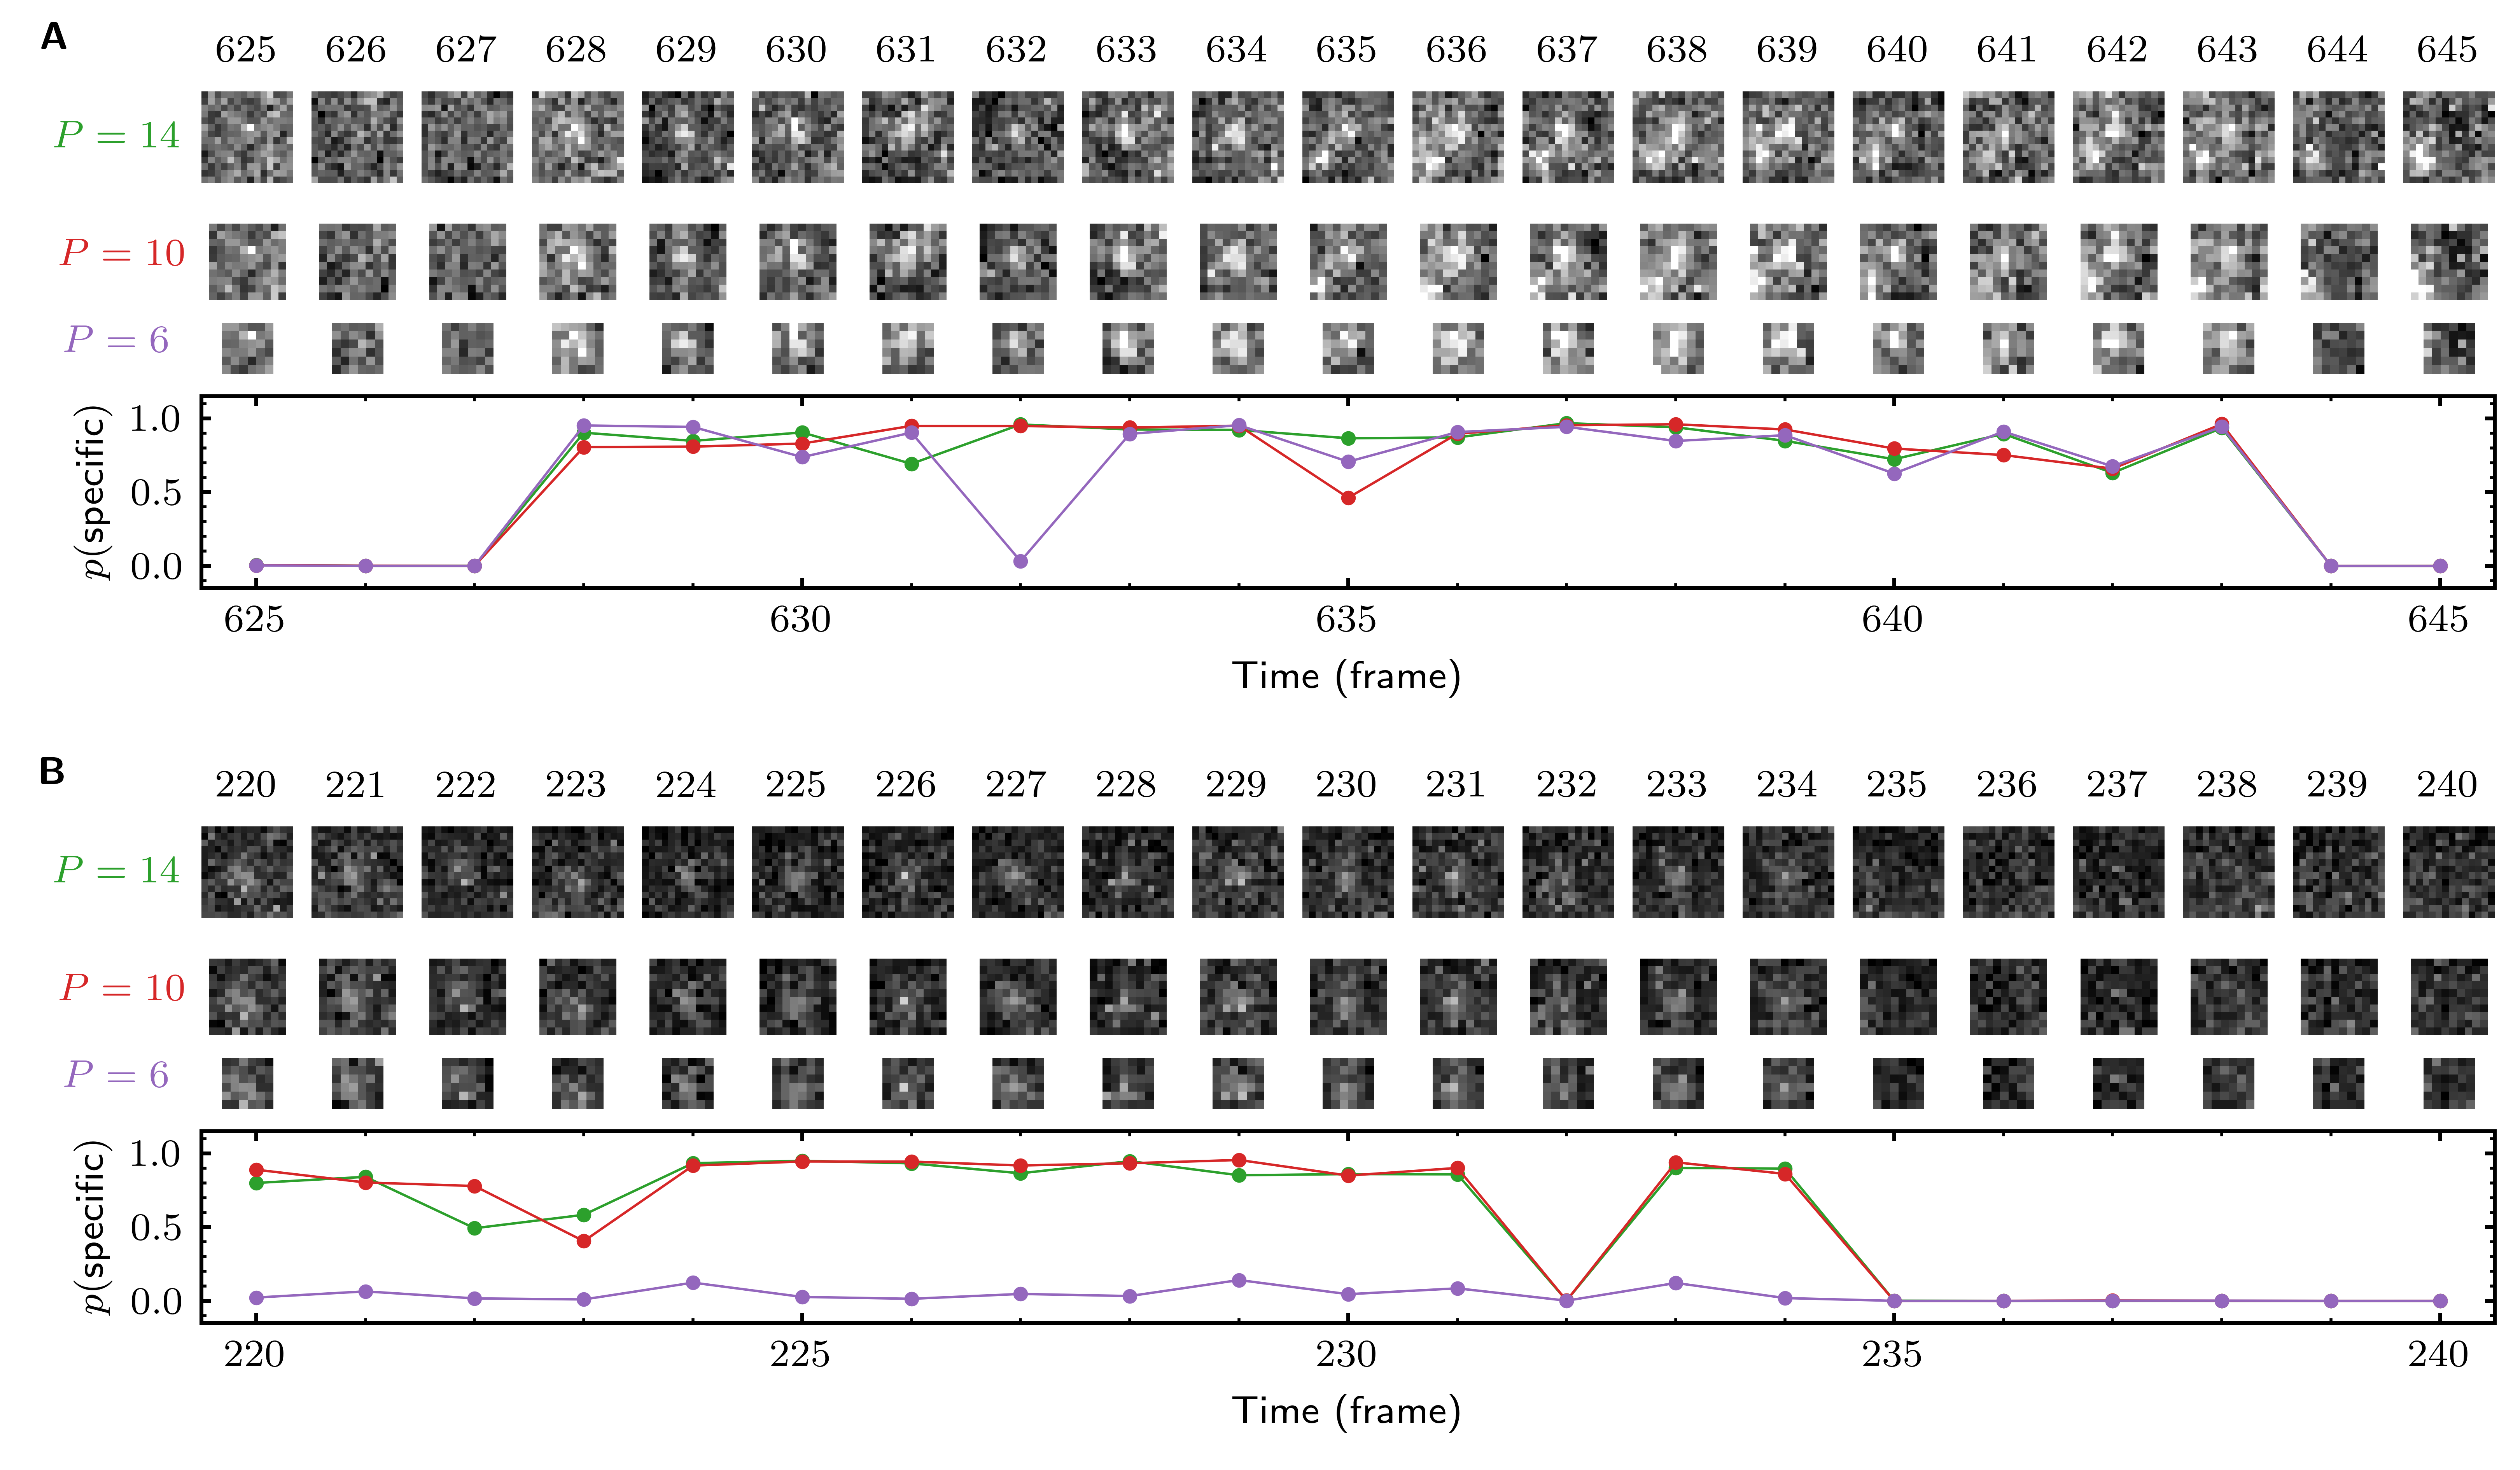
\includegraphics[width=183mm]{figures/tapqir_analysis_size.png}}\label{figsupp:size}
\end{fullwidth}
\end{figure}

\subsection{Tapqir robustly fits experimental data sets with different characteristics}

Next, we evaluated how well the model fits data sets encompassing a range of characteristics found in typical CoSMoS experiments. We analyzed four experimental data sets with varying SNR, frequency of target-specific spots, and frequencies of non-specific spots (\TABLE{datasets}). We then sampled AOI images from the posterior distributions of parameters (a method known as posterior predictive checking \citep{Gelman2013-ro}). These posterior predictive simulations accurately reproduce the experimental AOI appearances, recapitulating the noise characteristics and the numbers, intensities, shapes, and locations of spots (\FIGSUPP[tapqir_analysis]{ppc}, images).  The distributions of pixel intensities across the AOI are also closely reproduced (\FIGSUPP[tapqir_analysis]{ppc}, histograms) confirming that the noise model is accurate. Taken together, these results confirm that the model is rich enough to accurately capture the full range of image characteristics from CoSMoS data sets taken over different experimental conditions.  Importantly, all of the results on different experimental data sets were obtained using the same model (\FIG{graphical_model}D) and the same priors (Materials and Methods).  No tuning of the algorithm or prior measurement of data-set-specific properties was needed to achieve good fits for all data sets.

\subsection{Tapqir accuracy on simulated data with known global parameter values}

Next, we evaluated Tapqir's ability to reliably infer the values of global model parameters. To  accomplish this, we generated simulated data sets using a wide range of randomized parameter values and then fit the simulated data to the model (Supplementary File 2). Fit results show that global model parameters (i.e., average specific spot probability $\pi$, nonspecific binding density $\lambda$, proximity $\sigma^{xy}$, and gain $g$; see \FIG{graphical_model}D) are close to the simulated values (\FIGSUPP[tapqir_analysis]{randomized} and Supplementary File 2). This suggests that CoSMoS data contains enough information to reliably infer global model parameters and that the model is not obviously overparameterized. 

\subsection{Tapqir classification accuracy}

Having tested the basic function of the algorithm, we next turned to the key question of how accurately Tapqir can detect target-specific spots in data sets of increasing difficulty.

We first examined the accuracy of target-specific spot detection in simulated data sets with decreasing SNR (Supplementary File 3). By eye, spots can be readily discerned at SNR > 1 but cannot be clearly seen at SNR < 1 (\FIG{tapqir_performance}A). Tapqir gives similar or better performance:  if an image contains a target-specific spot, Tapqir correctly assigns it a target-specific spot probability $p(\mathsf{specific})$ that is on average close to one as long as SNR is adequate (i.e., SNR > 1) (\FIG{tapqir_performance}B).  In contrast, mean $p(\mathsf{specific})$ sharply decreases at SNR < 1, consistent with the subjective impression that no spot is recognized under those conditions.  In particular, images that contain a target-specific spot are almost always assigned a high $p(\mathsf{specific})$ for high SNR data and almost always assigned low $p(\mathsf{specific})$ for low SNR data (\FIG{tapqir_performance}C, green).  At marginal SNR $\simeq$ 1, these images are assigned a broad distribution of $p(\mathsf{specific})$ values, accurately reflecting the uncertainty in classifying such data.  Just as importantly, images with no target-specific spot are almost always assigned $p(\mathsf{specific}) < 0.5$, correctly reflecting the absence of the spot (\FIG{tapqir_performance}C, gray).

Ideally, we want to correctly identify target-specific binding when it occurs but also to avoid incorrectly identifying target-specific binding when it does not occur. To quantify Tapqir's classification accuracy, we next examined binary image classification statistics. Binary classification predictions were obtained by thresholding $p(\mathsf{specific})$ at $0.5$. We then calculated two complementary statistics: \textit{recall} and \textit{precision} \citep{Fawcett2006-bq} (\FIG{tapqir_performance}D; see Materials and Methods). Recall is defined as the fraction of true target-specific spots that are correctly predicted. Recall is high at high SNR and decreases at lower SNR. Recall is a binary analog of the mean $p(\mathsf{specific})$ for the subset of images containing target-specific spots; as expected the two quantities have similar dependencies on SNR (compare \FIG{tapqir_performance}B and \FIG{tapqir_performance}D, black). Precision is the fraction of predicted target-specific spots that are correctly predicted. Precision is near one at all SNR values tested (\FIG{tapqir_performance}D, red); this shows that the algorithm rarely misclassifies an image as containing a target-specific spot when none is present. 

In order to quantify the effects of both correctly and incorrectly classified images in a single statistic, we used the binary classification predictions to calculate the Matthews Correlation Coefficient (MCC) \citep{Matthews1975-rw} (see Materials and Methods). The MCC is equivalent to the Pearson correlation coefficient between the predicted and true classifications, giving 1 for a perfect match, 0 for a random match, and -1 for complete disagreement. The MCC results (\FIG{tapqir_performance}D, blue) suggest that the overall performance of Tapqir is excellent at SNR $\ge$ 1: the program rarely misses target-specific spots that are in reality present and rarely falsely reports a target-specific spot when none is present.  

The analyses of \FIG{tapqir_performance}B-D examined Tapqir performance on data in which the rate of target-nonspecific binding is moderate ($\lambda$ = 0.15 non-specific spots per AOI image on average).  We next examined the effects of increasing the non-specific rate.  In particular, we used simulated data (Supplementary File 1) with high SNR = 3.76 to test the classification accuracy of Tapqir at different non-specific binding densities up to $\lambda$ = 1, a value considerably higher than typical of usable experimental data (the experimental data sets in \TABLE{datasets} have $\lambda$ ranging from 0.04 to 0.30).   In analysis of these data sets, a few images with target-specific spots are misclassified as not having a specific spot ($p(\mathsf{specific})$ near zero) or as being ambiguous ($p(\mathsf{specific})$ near 0.5) (\FIG{tapqir_performance}F, green bars), and a few images with target-nonspecific spots are misclassified as having specific spot ($p(\mathsf{specific})$ near or above 0.5) (\FIG{tapqir_performance}F, gray bars), but these misclassifications only occurred at the unrealistically high $\lambda$ = 1 value.  Even in the simulation with this highest $\lambda$ value, Tapqir accurately identified target-specific spots (\FIG{tapqir_performance}E,F) and returned excellent binary classification statistics (\FIG{tapqir_performance}G). 

A weakness of some existing image-based CoSMoS spot discrimination methods is that target-nonspecific binding adjacent to a target-specific spot can interfere with correctly identifying the latter as target-specific.  The very high recall values obtained at $\lambda$ = 1 (\FIG{tapqir_performance}G) confirm that there are few such misidentifications by Tapqir even at high non-specific binding densities.  This good performance is likely facilitated by the feature of the Tapqir model that explicitly includes the possibility that both a specifically and a non-specifically bound spot may occur simultaneously in the same AOI. Consistent with this interpretation, we see effective detection of the specific and non-specific spots even in example AOIs in which the two spots are so closely spaced that they are not completely resolved (\FIG{tapqir_performance}H). In contrast, tests of existing CoSMoS image classification methods show that images with target-nonspecific spots are prone to misclassification.  As discussed previously \citep{Friedman2015-nx}, methods based on thresholding of integrated AOI intensities are prone to incorrectly classify target-nonspecific spots as target-specific.  Conversely, an existing ``spot-picker'' method based on empirical binary classification of 2-D AOI images \citep{Friedman2015-nx} is much more likely than Tapqir to fail to detect target specific spots when there is a nearby non-specific spot   (\FIGSUPP[tapqir_performance]{fn}).  This contributes to the superior overall performance we see for Tapqir vs. spot-picker on the $\lambda$ = 1 data set (recall 0.993 vs. 0.919; precision 0.943 vs. 0.873; MCC 0.961 vs. 0.874).

To further evaluate whether Tapqir is prone to misidentifying target-nonspecific spots as specific, we  simulated data sets with no target-specific binding at both low and high non-specific binding densities (Supplementary File 4). Analysis of such data (\FIG{tapqir_performance}I) shows that no target-specific binding (i.e., $p(\mathsf{specific}) > 0.6$) was detected even under the highest non-specific binding density, demonstrating that Tapqir is robust to false-positive target-specific spot detection even under these extreme conditions. 

\begin{figure}
\begin{fullwidth}
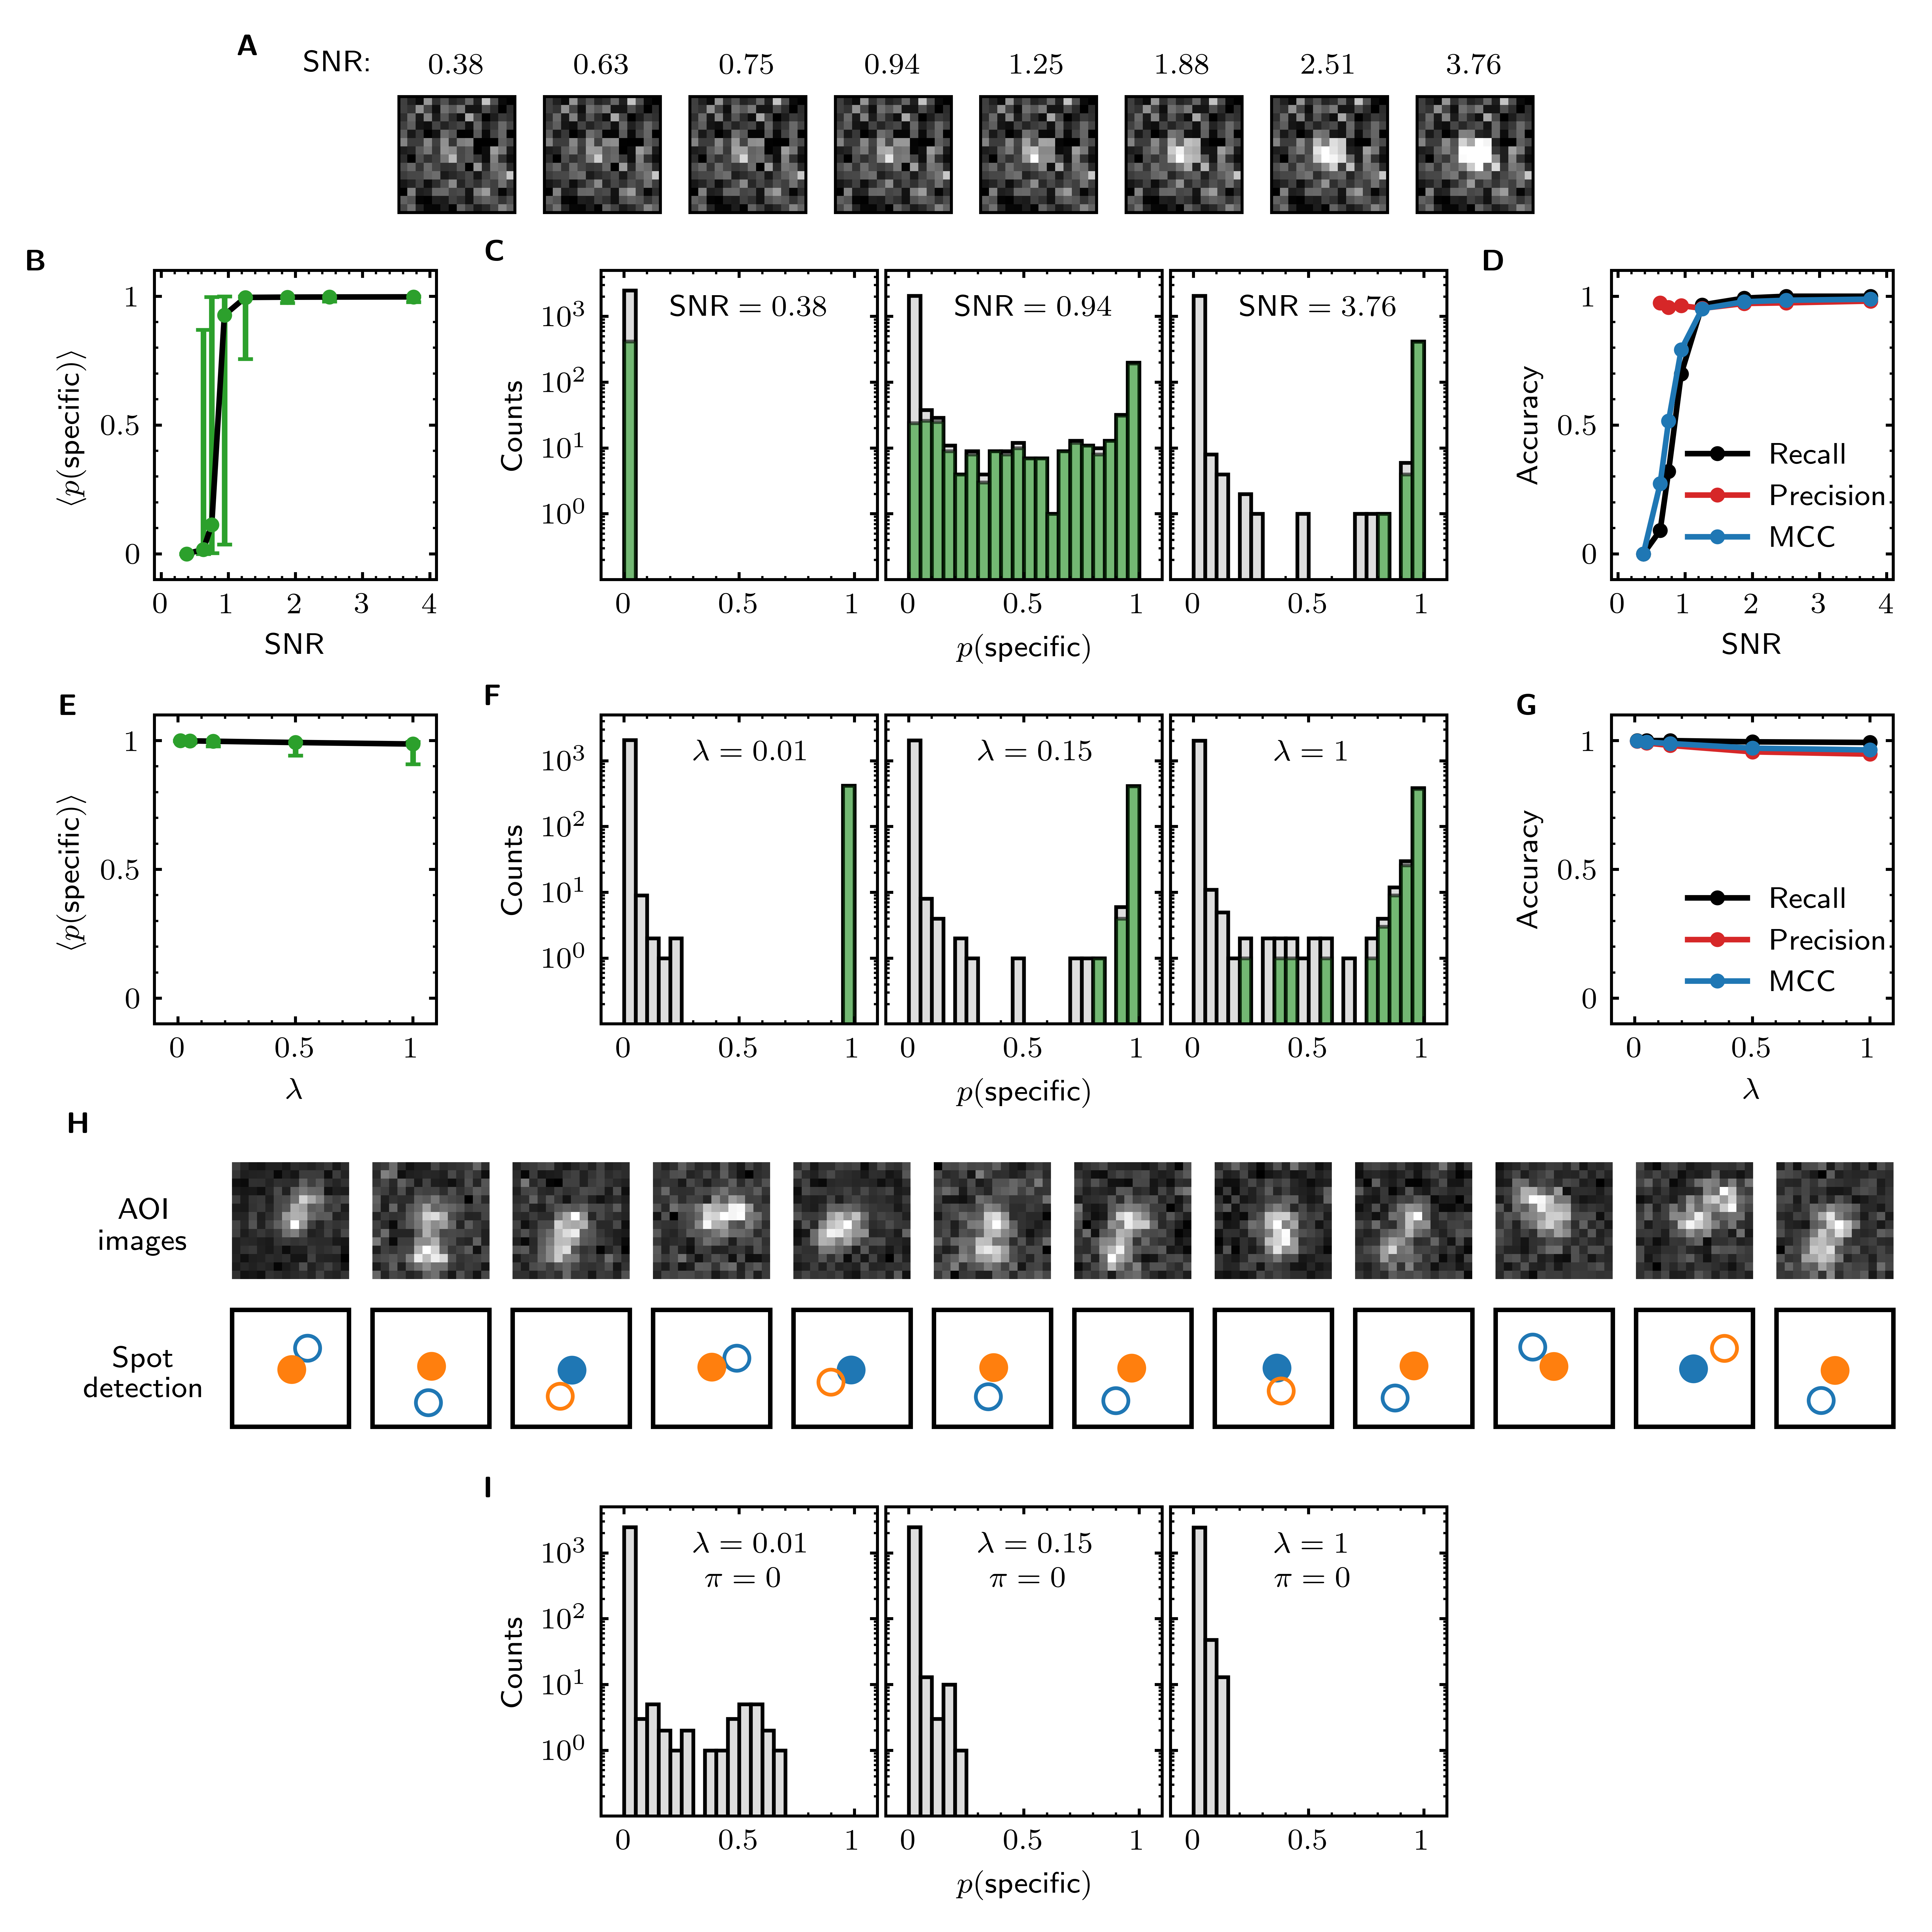
\includegraphics[width=183mm]{figures/tapqir_performance.png}
\caption{\textbf{Tapqir performance on simulated data with different SNRs or different non-specific binding rates.} (\textbf{A-D}) Analysis of simulated data over a range of SNR. SNR was varied in the simulations by changing spot intensity  $h$ while keeping other parameters constant (Supplemental Data 3). (\textbf{A}) Example images showing the appearance of the same target-specific spot simulated with increasing SNR.   (\textbf{B}) Mean of Tapqir-calculated target-specific spot probability $p(\mathsf{specific})$ (with 95\% high-density region; see Materials and Methods) for the subset of images where target-specific spots  are known to be present. (\textbf{C}) Histograms of $p(\mathsf{specific})$ for selected simulations with SNR indicated. Data are shown as stacked bars for images known to have (green, 15\%) or not have (gray, 85\%) target-specific spots.  Count is zero for bins where bars are not shown. (\textbf{D}) Accuracy of Tapqir image classification with respect to presence/absence of a target-specific spot. Accuracy was assessed by MCC, recall, and precision (see Results and Materials and Methods sections). (\textbf{E-G}) Same as in (\textbf{B-D}) but for the data simulated over a range of non-specific binding rates $\lambda$ at fixed SNR = 3.76 (Supplemental Data 1). (\textbf{H}) Spot recognition in AOI images containing closely spaced target-specific and non-specific spots.  Images were selected from the $\lambda = 1$ data set in e-g. AOI images and spot detection are plotted as in \FIG{tapqir_analysis}, with spot numbers 1 (blue) and 2 (orange) assigned arbitrarily and spots predicted to be target-specific shown as filled circles. (\textbf{I}) Same as in (\textbf{C}) but for the data simulated over a range of non-specific binding rates $\lambda$ with no target-specific binding ($\pi$ = 0) (Supplemental Data 4).}
\label{fig:tapqir_performance}
\figsupp[False negative misidentifications by Tapqir and spot-picker method.]{\textbf{False negative misidentifications by Tapqir and spot-picker method.} The same $\lambda$ = 1 simulated data set used in \FIG{tapqir_performance}E-H (\texttt{lamda1} in Supplemental Data 1) was analyzed by Tapqir and spot-picker.  The data set contained 418 AOI images containing target-specific spots, of which the 37 shown here were falsely predicted to contain no target-specific spot (3 by Tapqir and 34 by spot-picker). Correct ($+$) and incorrect ($-$) predictions by each program are indicated. In all AOI images except AOI 3 frame 109, there is a nearby target-nonspecific spot in addition to the target-specific one. False negative classifications by spot-picker method are presumably due to the presence of a closely located target-nonspecific spot that distorts the shape of a target-specific spot. Tapqir, on the other hand, is able to correctly infer the presence of two closely located spots even when they are not completely resolved (\FIG{tapqir_performance}H). The rare (3 out of 418) false negative classifications by Tapqir likely arise from target-specific spots with centers that deviate from the target location by much more ($\sim$ 0.7 pixels) than the inferred proximity parameter ($\sigma^{xy}$ = 0.2 pixels).}{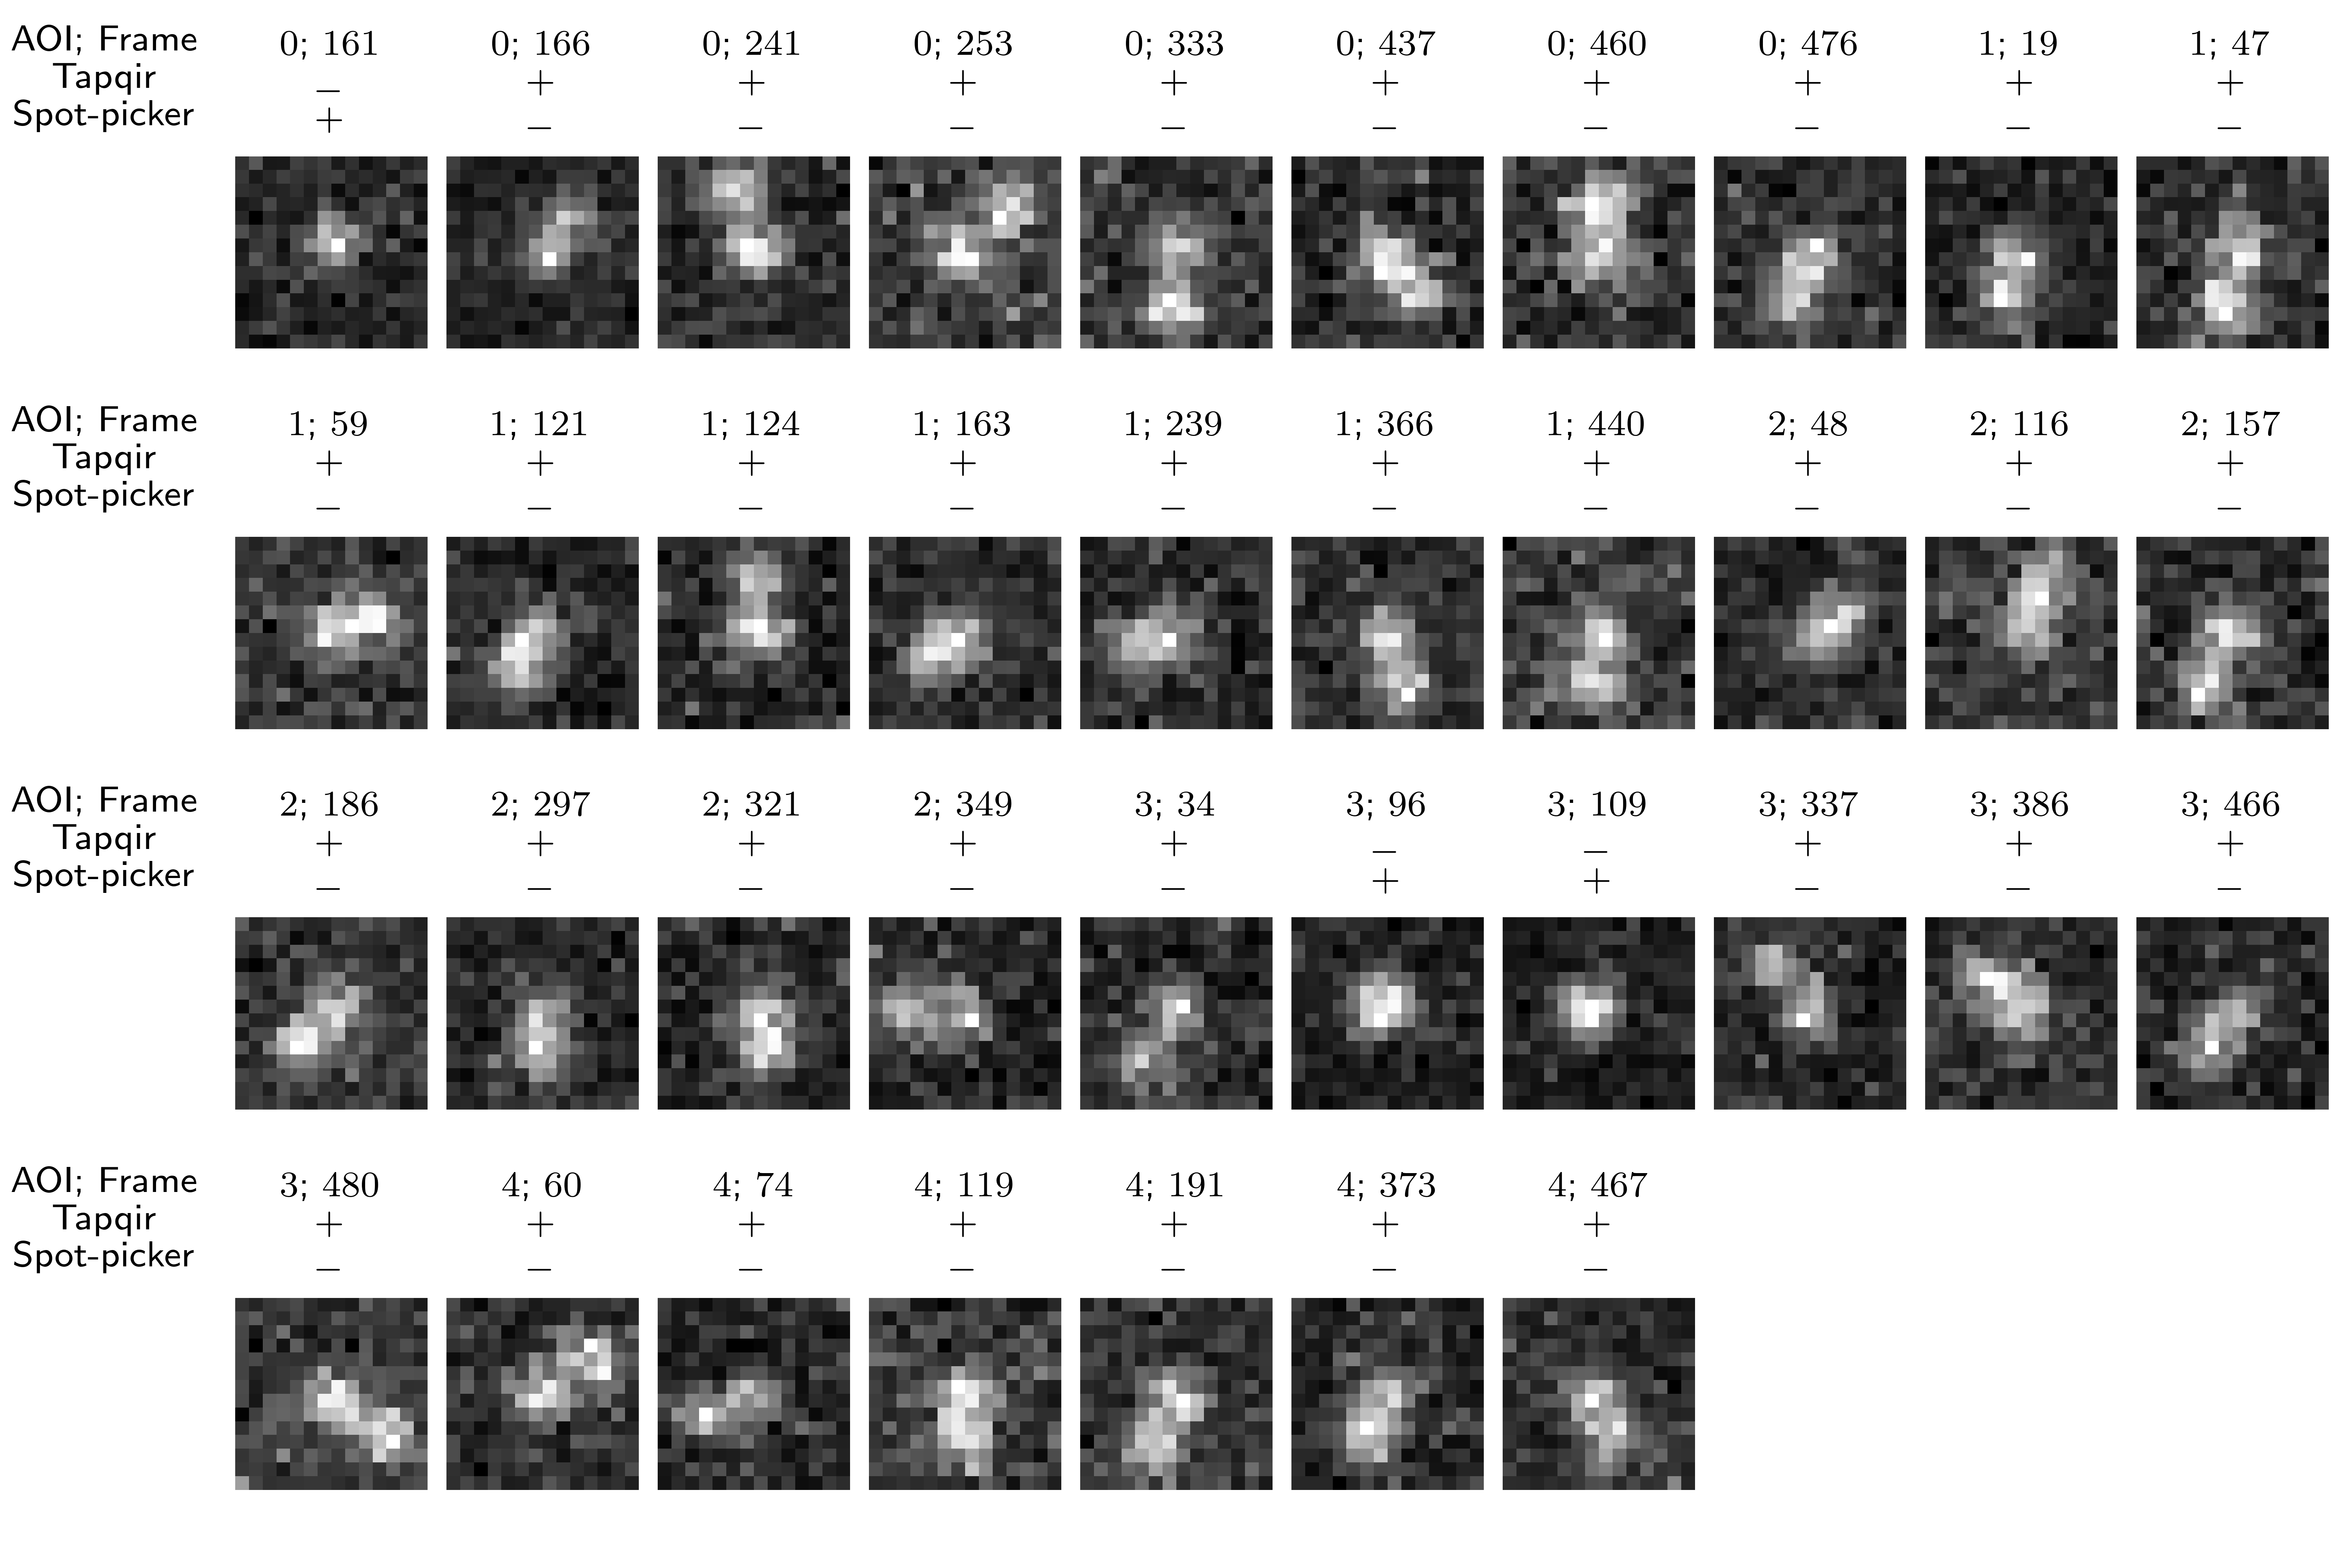
\includegraphics[width=183mm]{figures/tapqir_performance_fn.png}}\label{figsupp:fn}
\end{fullwidth}
\end{figure}

Since target-nonspecific spots are built into the \emph{cosmos} model, there is no need to choose excessively small AOIs in an attempt to exclude non-specific spots from analysis. We found that reducing AOI size (from 14 x 14 to 6 x 6 pixels) did not appreciably affect analysis accuracy on simulated data (\TABLE{aoisize}). In analysis of experimental data, smaller AOI sizes caused occasional changes in calculated $p(\mathsf{specific})$ values reflecting apparent missed detection of a few spots (\FIGSUPP[tapqir_analysis]{size}). Out of caution, we therefore used 14 x 14 pixel AOIs routinely, even though the larger AOIs somewhat reduced computation speed (\TABLE{aoisize} and \FIGSUPP[tapqir_analysis]{size}).

\subsection{Kinetic and thermodynamic analysis of molecular interactions}

The most widespread application of CoSMoS experiments is to measure rate and equilibrium constants for the binding interaction of the target and binder molecules being studied.  We next tested whether these constants can be accurately determined using Tapqir-calculated posterior predictions. 

We first simulated CoSMoS data sets (Supplementary File 5) that reproduced the behavior of a one-step association/dissociation reaction mechanism (\FIG{kinetic_analysis}A and \FIG{kinetic_analysis}B, blue). Simulated data were analyzed with Tapqir yielding $p(\mathsf{specific})$ values for each frame (e.g., \FIG{kinetic_analysis}B, green). We wanted to estimate rate constants using the full information contained in the $p(\mathsf{specific})$ probabilities, so we did not simply threshold $p(\mathsf{specific})$ for this analysis.  Instead, from each single-AOI $p(\mathsf{specific})$ time record we constructed a family of binary time records (\FIG{kinetic_analysis}B, black) by Monte Carlo sampling according to the  $p(\mathsf{specific})$ time series. Each family member has well-defined target-specific binder-present and binder-absent intervals $\Delta t_\mathsf{on}$ and $\Delta t_\mathsf{off}$, respectively. Each of these time records was then analyzed with a two-state hidden Markov model (HMM) (see Materials and Methods), producing a distribution of inferred rate constants from which we calculated mean values and their uncertainties (\FIG{kinetic_analysis}C,D). Comparison of the simulated and inferred values shows that both $k_\mathsf{on}$ and $k_\mathsf{off}$ rate constants are accurate within 30\% at nonspecific binding densities typical of experimental data ($\lambda \leq$ 0.5). At higher nonspecific binding densities, rare interruptions caused by false-positive and false-negative spot detection shorten $\Delta t_\mathsf{on}$ and $\Delta t_\mathsf{off}$ distributions, leading to moderate systematic overestimation of the association and dissociation rate constants.

From the same simulated data we calculated the equilibrium constant $K_\mathsf{eq}$ and its uncertainty. This calculation does not require a time-dependent model and can be obtained directly from the posterior distribution of the average specific-binding probability $\pi$. The estimated equilibrium constants are highly accurate even at excessively high values of $\lambda$ (\FIG{kinetic_analysis}E).  The high accuracy results from the fact that equilibrium constant measurements in general are much less affected than kinetic measurements by occasional false positives and false negatives in spot detection. 

The forgoing analysis shows that Tapqir can accurately recover kinetic and thermodynamic constants from simulated CoSMoS data.  However, experimental CoSMoS data sets can be more diverse.  In addition to having different SNR and non-specific binding frequency values, they also may have non-idealities in spot shape (caused by optical aberrations) and in noise (caused by molecular diffusion in and out of the TIRF evanescent field).  In order to see if Tapqir analysis is robust to these and other properties of real experimental data, we analyzed several CoSMoS data sets taken from different experimental projects. Analysis of each data set took a few hours of computation time on a GPU-equipped desktop computer or cloud computing service (\TABLE{datasets}). We first visualized the results as probabilistic rastergrams (\FIG{experimental_data}A, \FIGSUPP[experimental_data]{DatasetA}A, \FIGSUPP[experimental_data]{DatasetC}A, and \FIGSUPP[experimental_data]{DatasetD}A), in which each horizontal line represents the time record from a single AOI.  Unlike the binary spot/no-spot rastergrams in previous studies (e.g., \cite{Friedman2013-sf,Rosen2020-zn}) we plotted the Tapqir-calculated spot probability $p(\mathsf{specific})$ using a color scale.  This representation allows a more nuanced understanding of the data.  For example, \FIG{experimental_data}A reveals that while the long-duration spot detection events typically are assigned a high probability (yellow), some of the shortest duration events have an intermediate $p(\mathsf{specific})$ (green) indicating that the assignment of these as target-specific is uncertain.  

\begin{figure}
\begin{fullwidth}
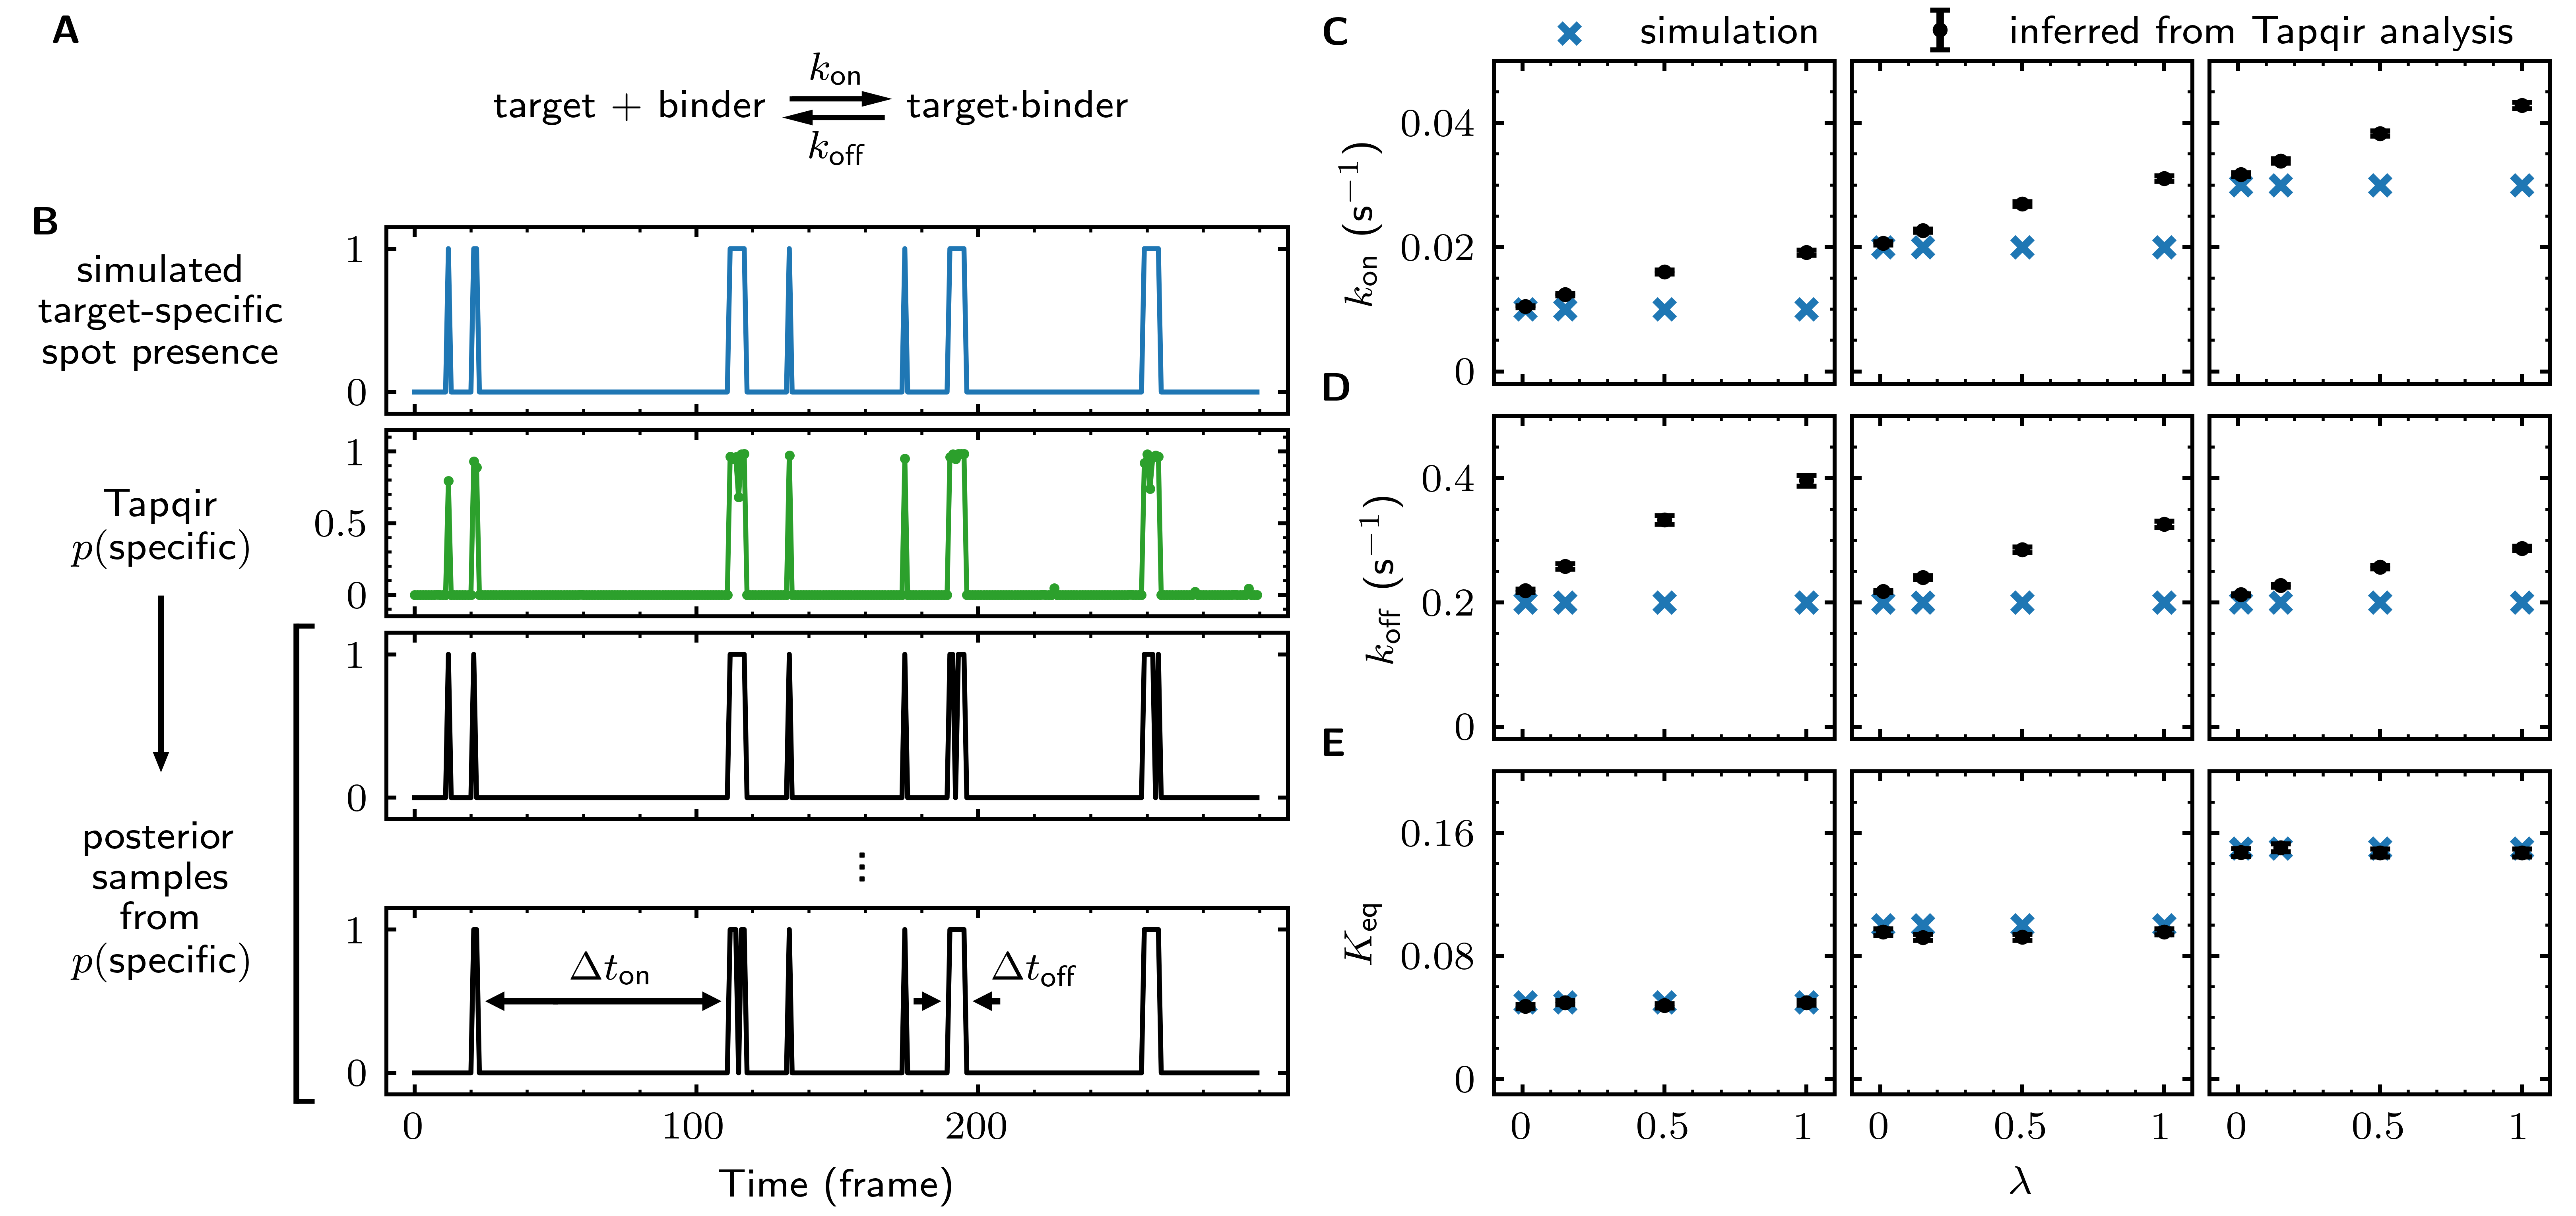
\includegraphics[width=183mm]{figures/kinetic_analysis.png}
\caption{\textbf{Tapqir analysis of association/dissociation kinetics and thermodynamics.} (\textbf{A}) Chemical scheme for a one-step association/dissociation reaction at equilibrium with apparent first-order binding and dissociation rate constants $k_{\mathsf{on}}$ and $k_{\mathsf{off}}$, respectively. (\textbf{B}) A simulation of the reaction in (\textbf{A}) and scheme for kinetic analysis with Tapqir. Simulation used SNR = 3.76, $k_\mathsf{on}$ = 0.02 s$^{-1}$, $k_\mathsf{off}$ = 0.2 s$^{-1}$, and a high target-nonspecific binding frequency $\lambda$ = 1 (Supplemental Data 5, data set \texttt{kon0.02lamda1}). Full dataset consists of 100 AOI locations and 1000 frames each for on-target data and off-target control data. Shown is a short extract of on-target data from a single AOI location in the simulation.  Plots show simulated presence/absence of the target-specific spot (blue) and Tapqir-calculated estimate of corresponding target-specific spot probability $p(\mathsf{specific})$ (green). Two thousand binary traces (e.g., black records) were sampled from the $p(\mathsf{specific})$ posterior distribution and used to infer $k_\mathsf{on}$ and $k_\mathsf{off}$ using a two-state hidden Markov model (HMM) (see Materials and Methods). Each sample trace contains well-defined time intervals corresponding to target-specific spot presence and absence (e.g., $\Delta t_\mathsf{on}$ and $\Delta t_\mathsf{off}$). (\textbf{C,D,E}) Kinetic and equilibrium constants from simulations (Supplemental Data 5) using a range of $k_\mathsf{on}$ values and  target-nonspecific spot frequencies $\lambda$, with constant $k_\mathsf{off}$ = 0.2 s$^{-1}$. (\textbf{C}) Values of $k_{\mathsf{on}}$ used in simulations (blue) and mean values (and 95\% CIs, black) inferred by HMM analysis from the 2000 posterior samples.  Some error bars are smaller than the points and thus not visible. (\textbf{D}) Same as (\textbf{C}) but for $k_{\mathsf{off}}$. (\textbf{E})  Binding equilibrium constants $K_{\mathsf{eq}} = k_{\mathsf{on}} / k_{\mathsf{off}}$ used in simulation (blue) and inferred from Tapqir-calculated $\pi$ as $K_{\mathsf{eq}} = \pi / (1 - \pi)$ (black). }
\label{fig:kinetic_analysis}
\end{fullwidth}
\end{figure}

To demonstrate the utility of Tapqir for kinetic analysis of real experimental data, we measured binder association rate constants in previously published experimental data sets (\TABLE{datasets}).  We employed our previous strategy  \citep{Friedman2012-if,Friedman2015-nx} of analyzing the duration of the binder-absent intervals that preceded the first binding event.  Such time-to-first binding analysis improves the accuracy of association rate constant estimates relative to those obtained by analyzing all $\Delta t_\mathsf{off}$ values by minimizing the effects of target molecules occupied by photobleached binders, dye blinking and false negative dropouts that occur within a continuous binder dwell interval.  To perform a time-to-first-binding analysis using Tapqir, we used the posterior sampling method (as in \FIG{kinetic_analysis}B, black records) to determine the initial $\Delta t_\mathsf{off}$ in each AOI record. These data were fit to a kinetic model \citep{Friedman2012-if,Friedman2015-nx} in which only a fraction of target molecules $A_\mathsf{f}$ were binding competent and which includes both exponential target-specific association with rate constant $k_\mathsf{a}$, as well as exponential non-specific association with rate constant $k_\mathsf{ns}$ (\FIG{experimental_data}B, \FIGSUPP[experimental_data]{DatasetA}B, \FIGSUPP[experimental_data]{DatasetC}B, and \FIGSUPP[experimental_data]{DatasetD}B).  The Tapqir-derived fits showed excellent agreement with the kinetic model.  

To further assess the utility of the Tapqir method, we used experimental data sets and compared the Tapqir association kinetics results with those from the previously published empirical binary ``spot-picker'' method \citep{Friedman2015-nx} (\FIG{experimental_data}C, \FIGSUPP[experimental_data]{DatasetA}C, \FIGSUPP[experimental_data]{DatasetC}C, and \FIGSUPP[experimental_data]{DatasetD}C). The values of the association rate constant $k_\mathsf{a}$ obtained using these two methods are in good agreement with each other (\FIG{experimental_data}D, \FIGSUPP[experimental_data]{DatasetA}D, \FIGSUPP[experimental_data]{DatasetC}D, and \FIGSUPP[experimental_data]{DatasetD}D). We emphasize that while Tapqir is fully objective, achieving these results with the spot-picker method required optimization by subjective adjustment of spot detection thresholds.  We noted some differences between the two methods in the non-specific association rate constants $k_\mathsf{ns}$. Differences are expected because these parameters are defined differently in the different non-specific binding models used in Tapqir and  spot-picker (see Materials and Methods).

\begin{figure}
\begin{fullwidth}
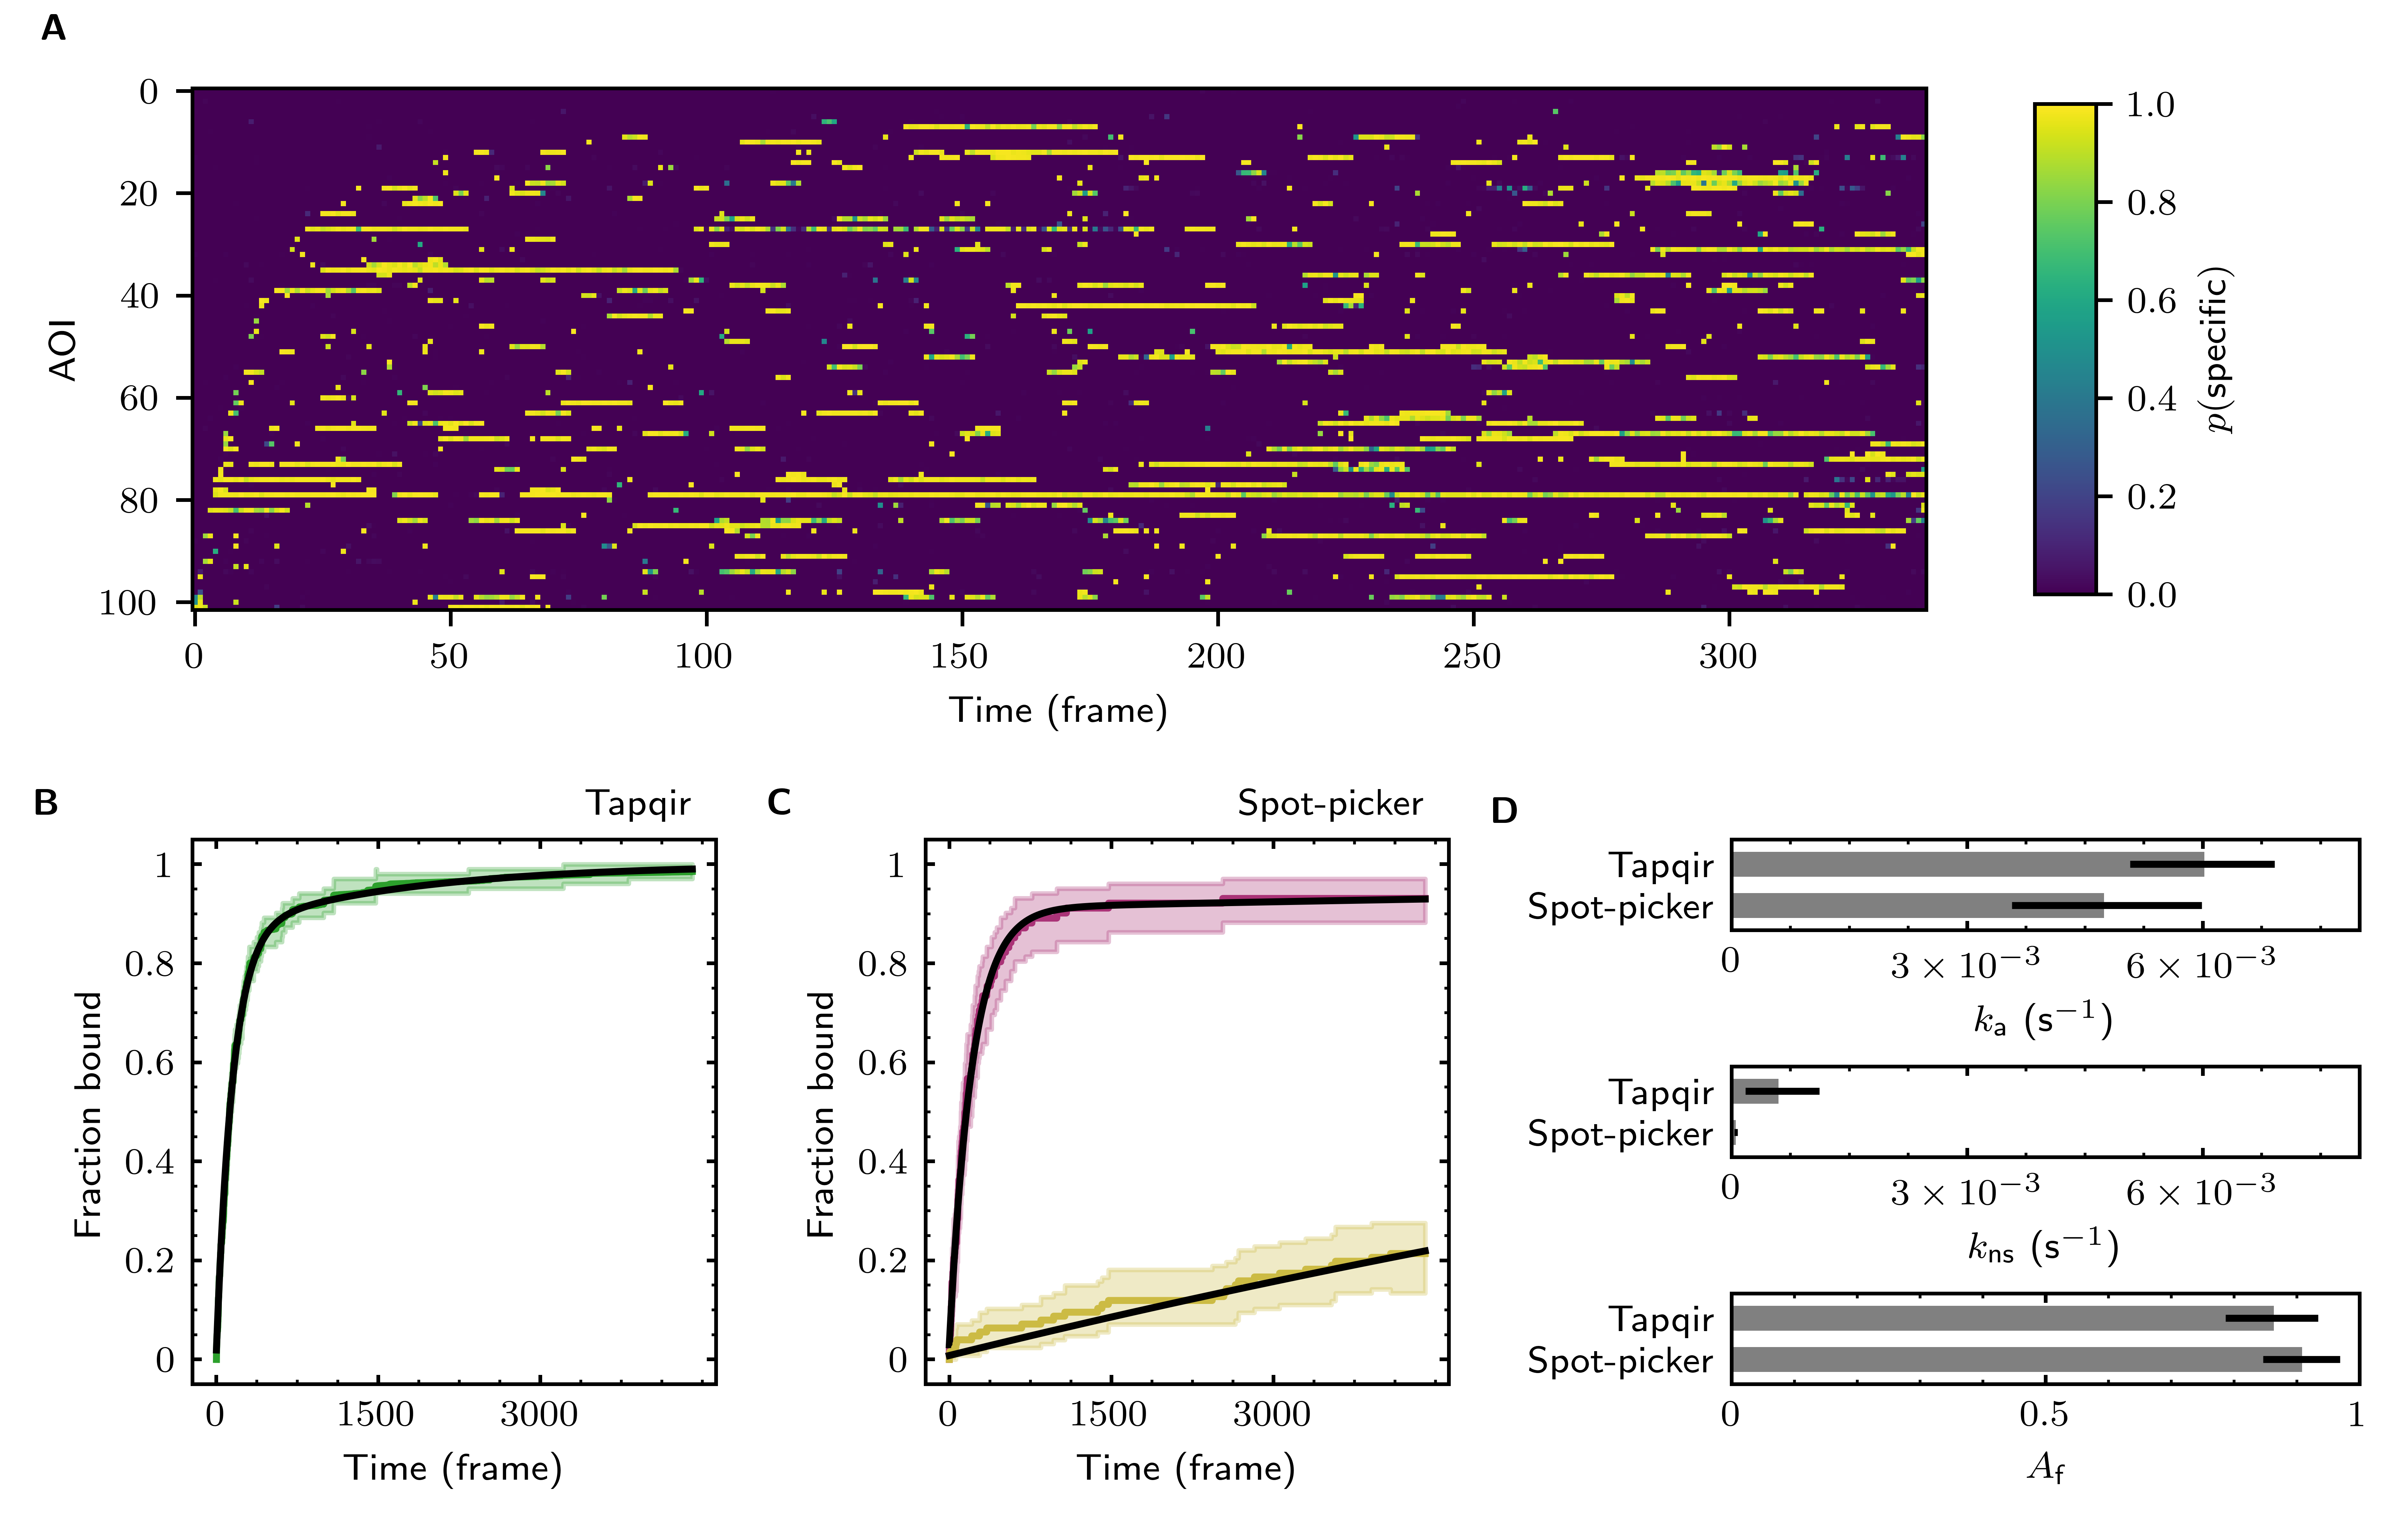
\includegraphics[width=183mm]{figures/experimental_data.png}
\caption{\textbf{Extraction of target-binder association kinetics from example experimental data.} Data are from Data set B ($\mathrm{SNR} = 3.43$, $\lambda = 0.1290$; see \TABLE{datasets}).  (\textbf{A}) Probabilistic rastergram representation of Tapqir-calculated target-specific spot  probabilities $p(\mathsf{specific})$ (color scale). AOIs were ordered by decreasing times-to-first-binding. For clarity, only every thirteenth frame is plotted. (\textbf{B}) Time-to-first-binding distribution using Tapqir. Plot shows the cumulative fraction of AOIs that exhibited one or more target-specific binding events by the indicated frame number (green) and fit curve (black). Shading indicates uncertainty. (\textbf{C}) Time-to-first-binding distribution using an empirical spot-picker method \cite{Friedman2013-sf}. The spot-picker method jointly fits first spots observed in off-target control AOIs (yellow) and in on-target AOIs (purple) with fit curves (black). (\textbf{D}) Values of kinetic parameters  $k_\mathsf{a}$, $k_\mathsf{ns}$, and $A_\mathsf{f}$ (see text) derived from fits in (\textbf{B}) and (\textbf{C}). Uncertainties reported in (\textbf{B, C, D}) represent 95\% credible intervals for Tapqir and 95\% confidence intervals for spot-picker (see Methods).
}
\label{fig:experimental_data}
\figsupp[Additional example showing extraction of target-binder association kinetics from experimental data.]{\textbf{Additional example showing extraction of target-binder association kinetics from experimental data.} Data are from Data set A ($\mathrm{SNR} = 1.63$, $\lambda = 0.2958$; see \TABLE{datasets}).  Results are plotted as in \FIG{experimental_data}, except that for clarity only every $2^\mathrm{nd}$ frame and every $3^\mathrm{rd}$ AOI is shown in (\textbf{A}).}{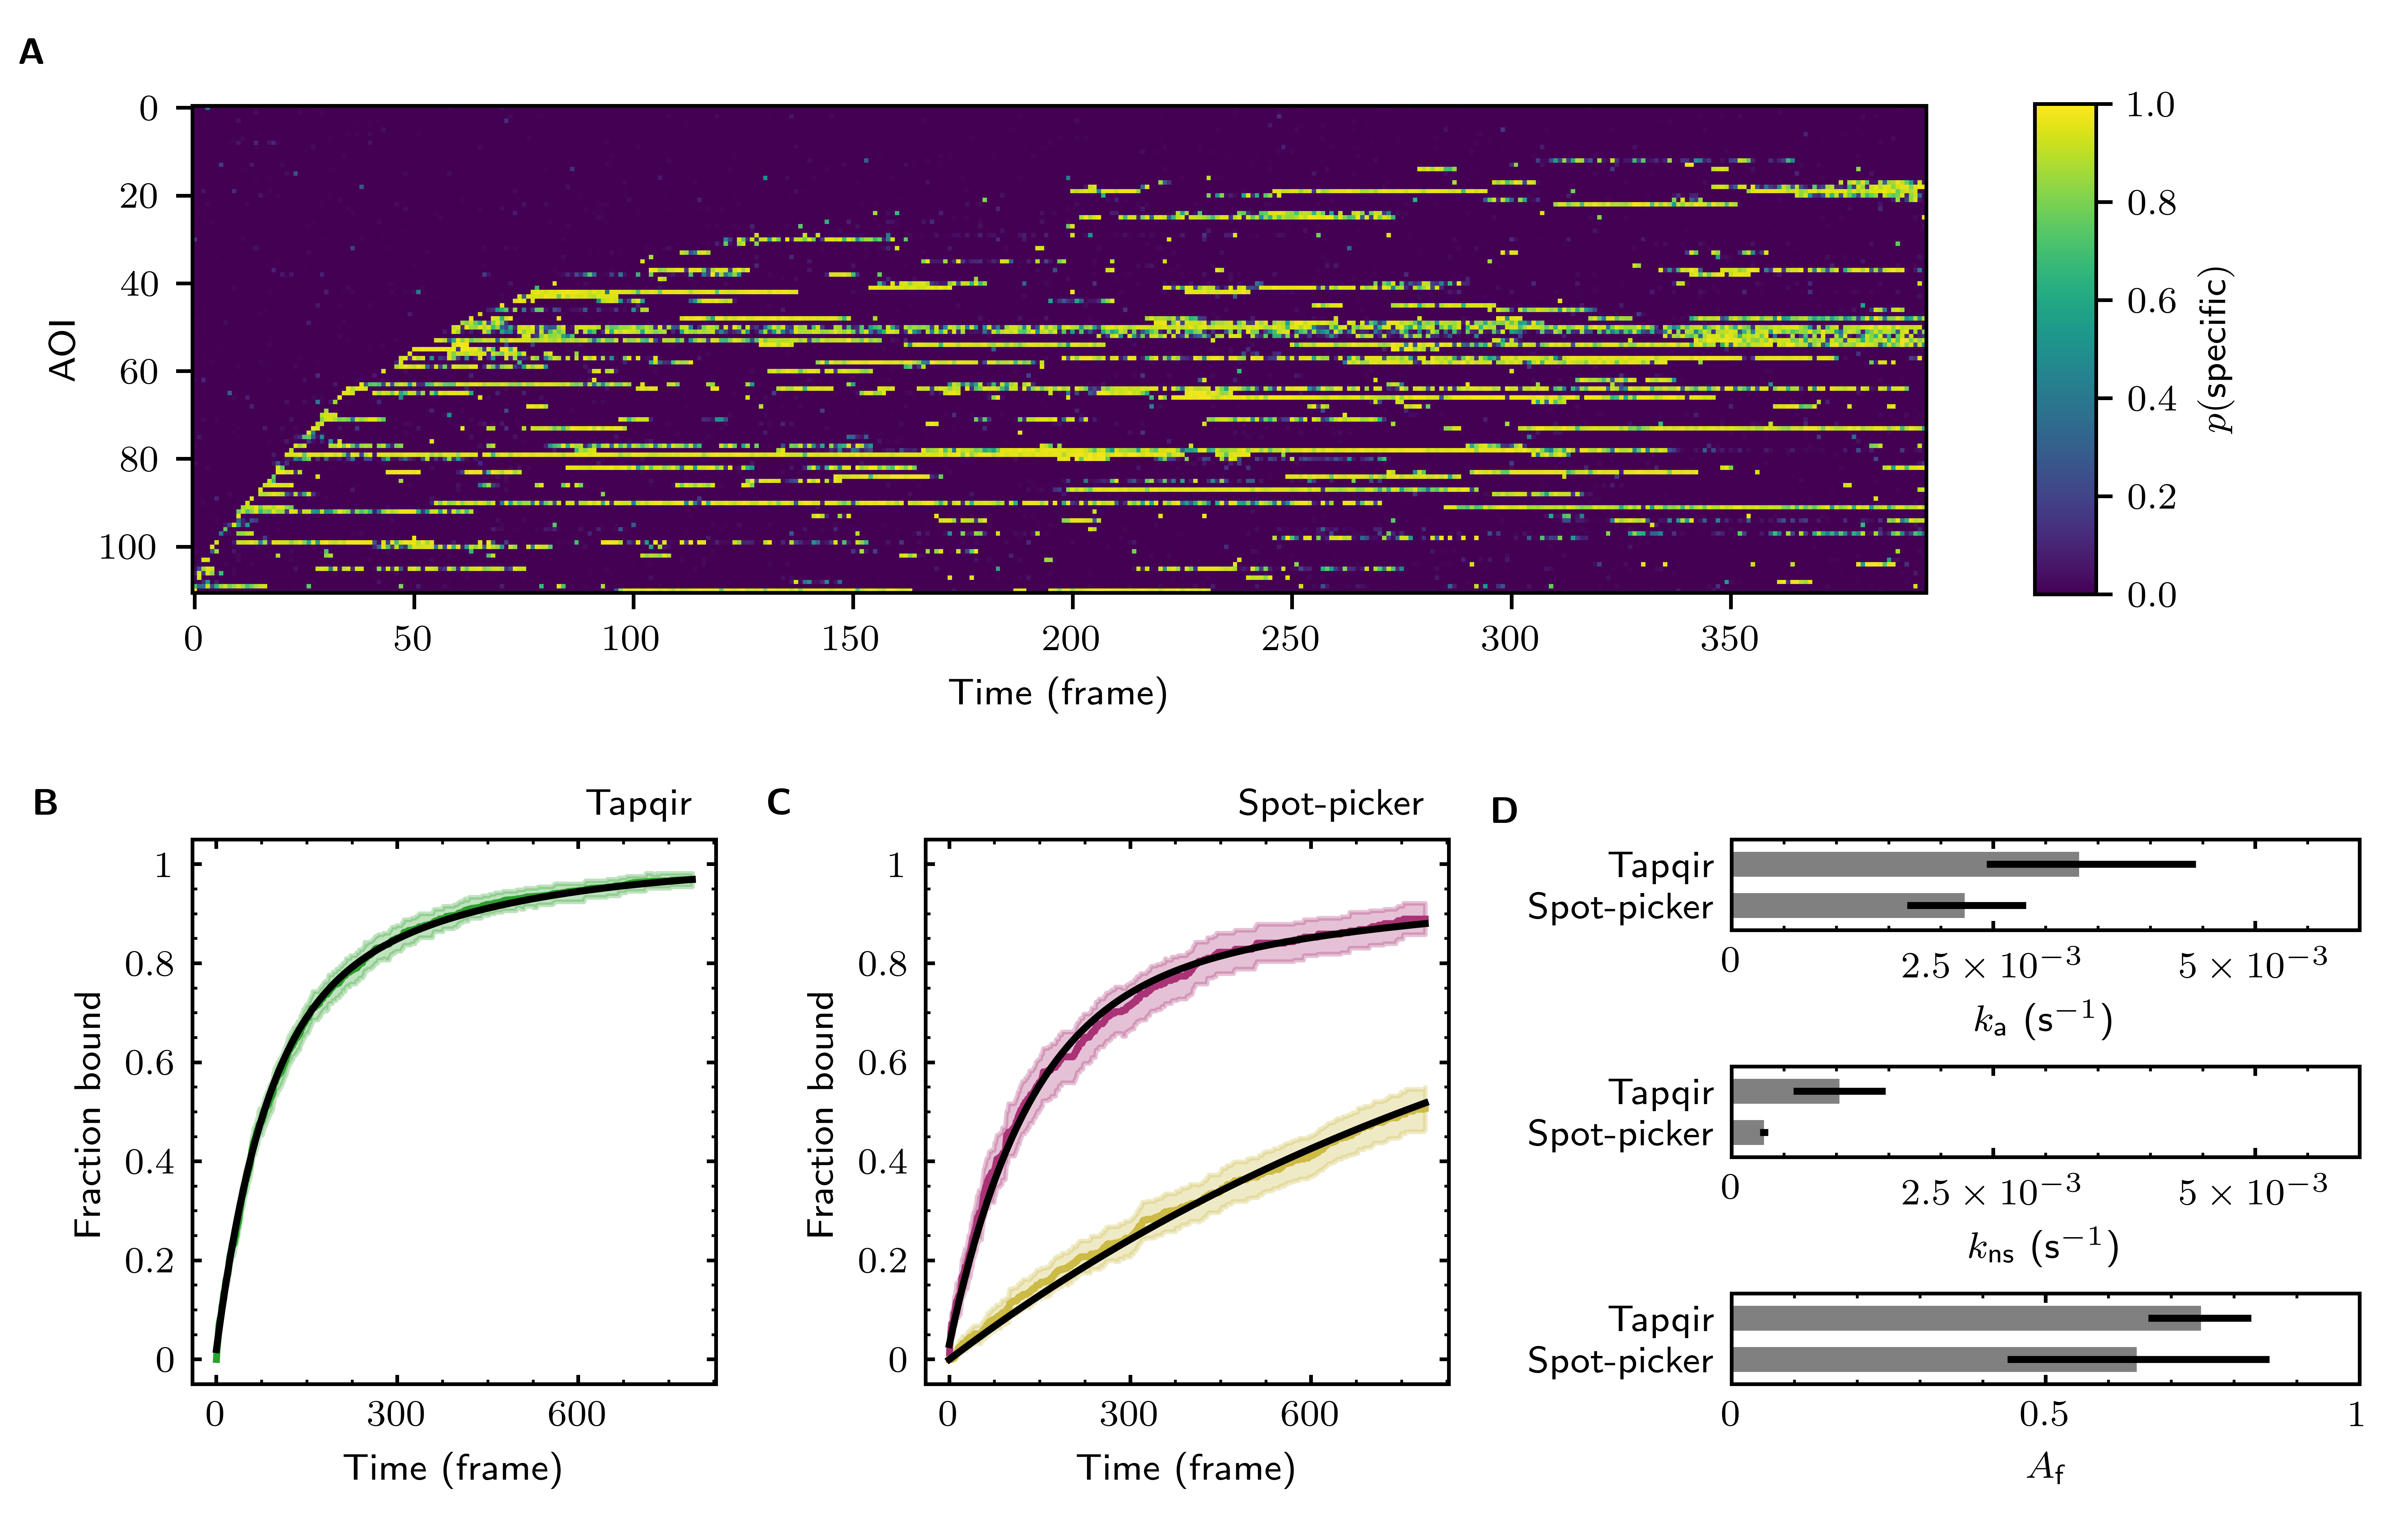
\includegraphics[width=183mm]{figures/experimental_data_DatasetA.png}}\label{figsupp:DatasetA}

\figsupp[Additional example showing extraction of target-binder association kinetics from experimental data.]{\textbf{Additional example showing extraction of target-binder association kinetics from experimental data.} Data are from Data set C ($\textrm{SNR} = 4.18$, $\lambda = 0.0716$; see \TABLE{datasets}).  Results are plotted as in \FIG{experimental_data}, except that for clarity only every $10^\mathrm{th}$ AOI is shown in (\textbf{A}).}{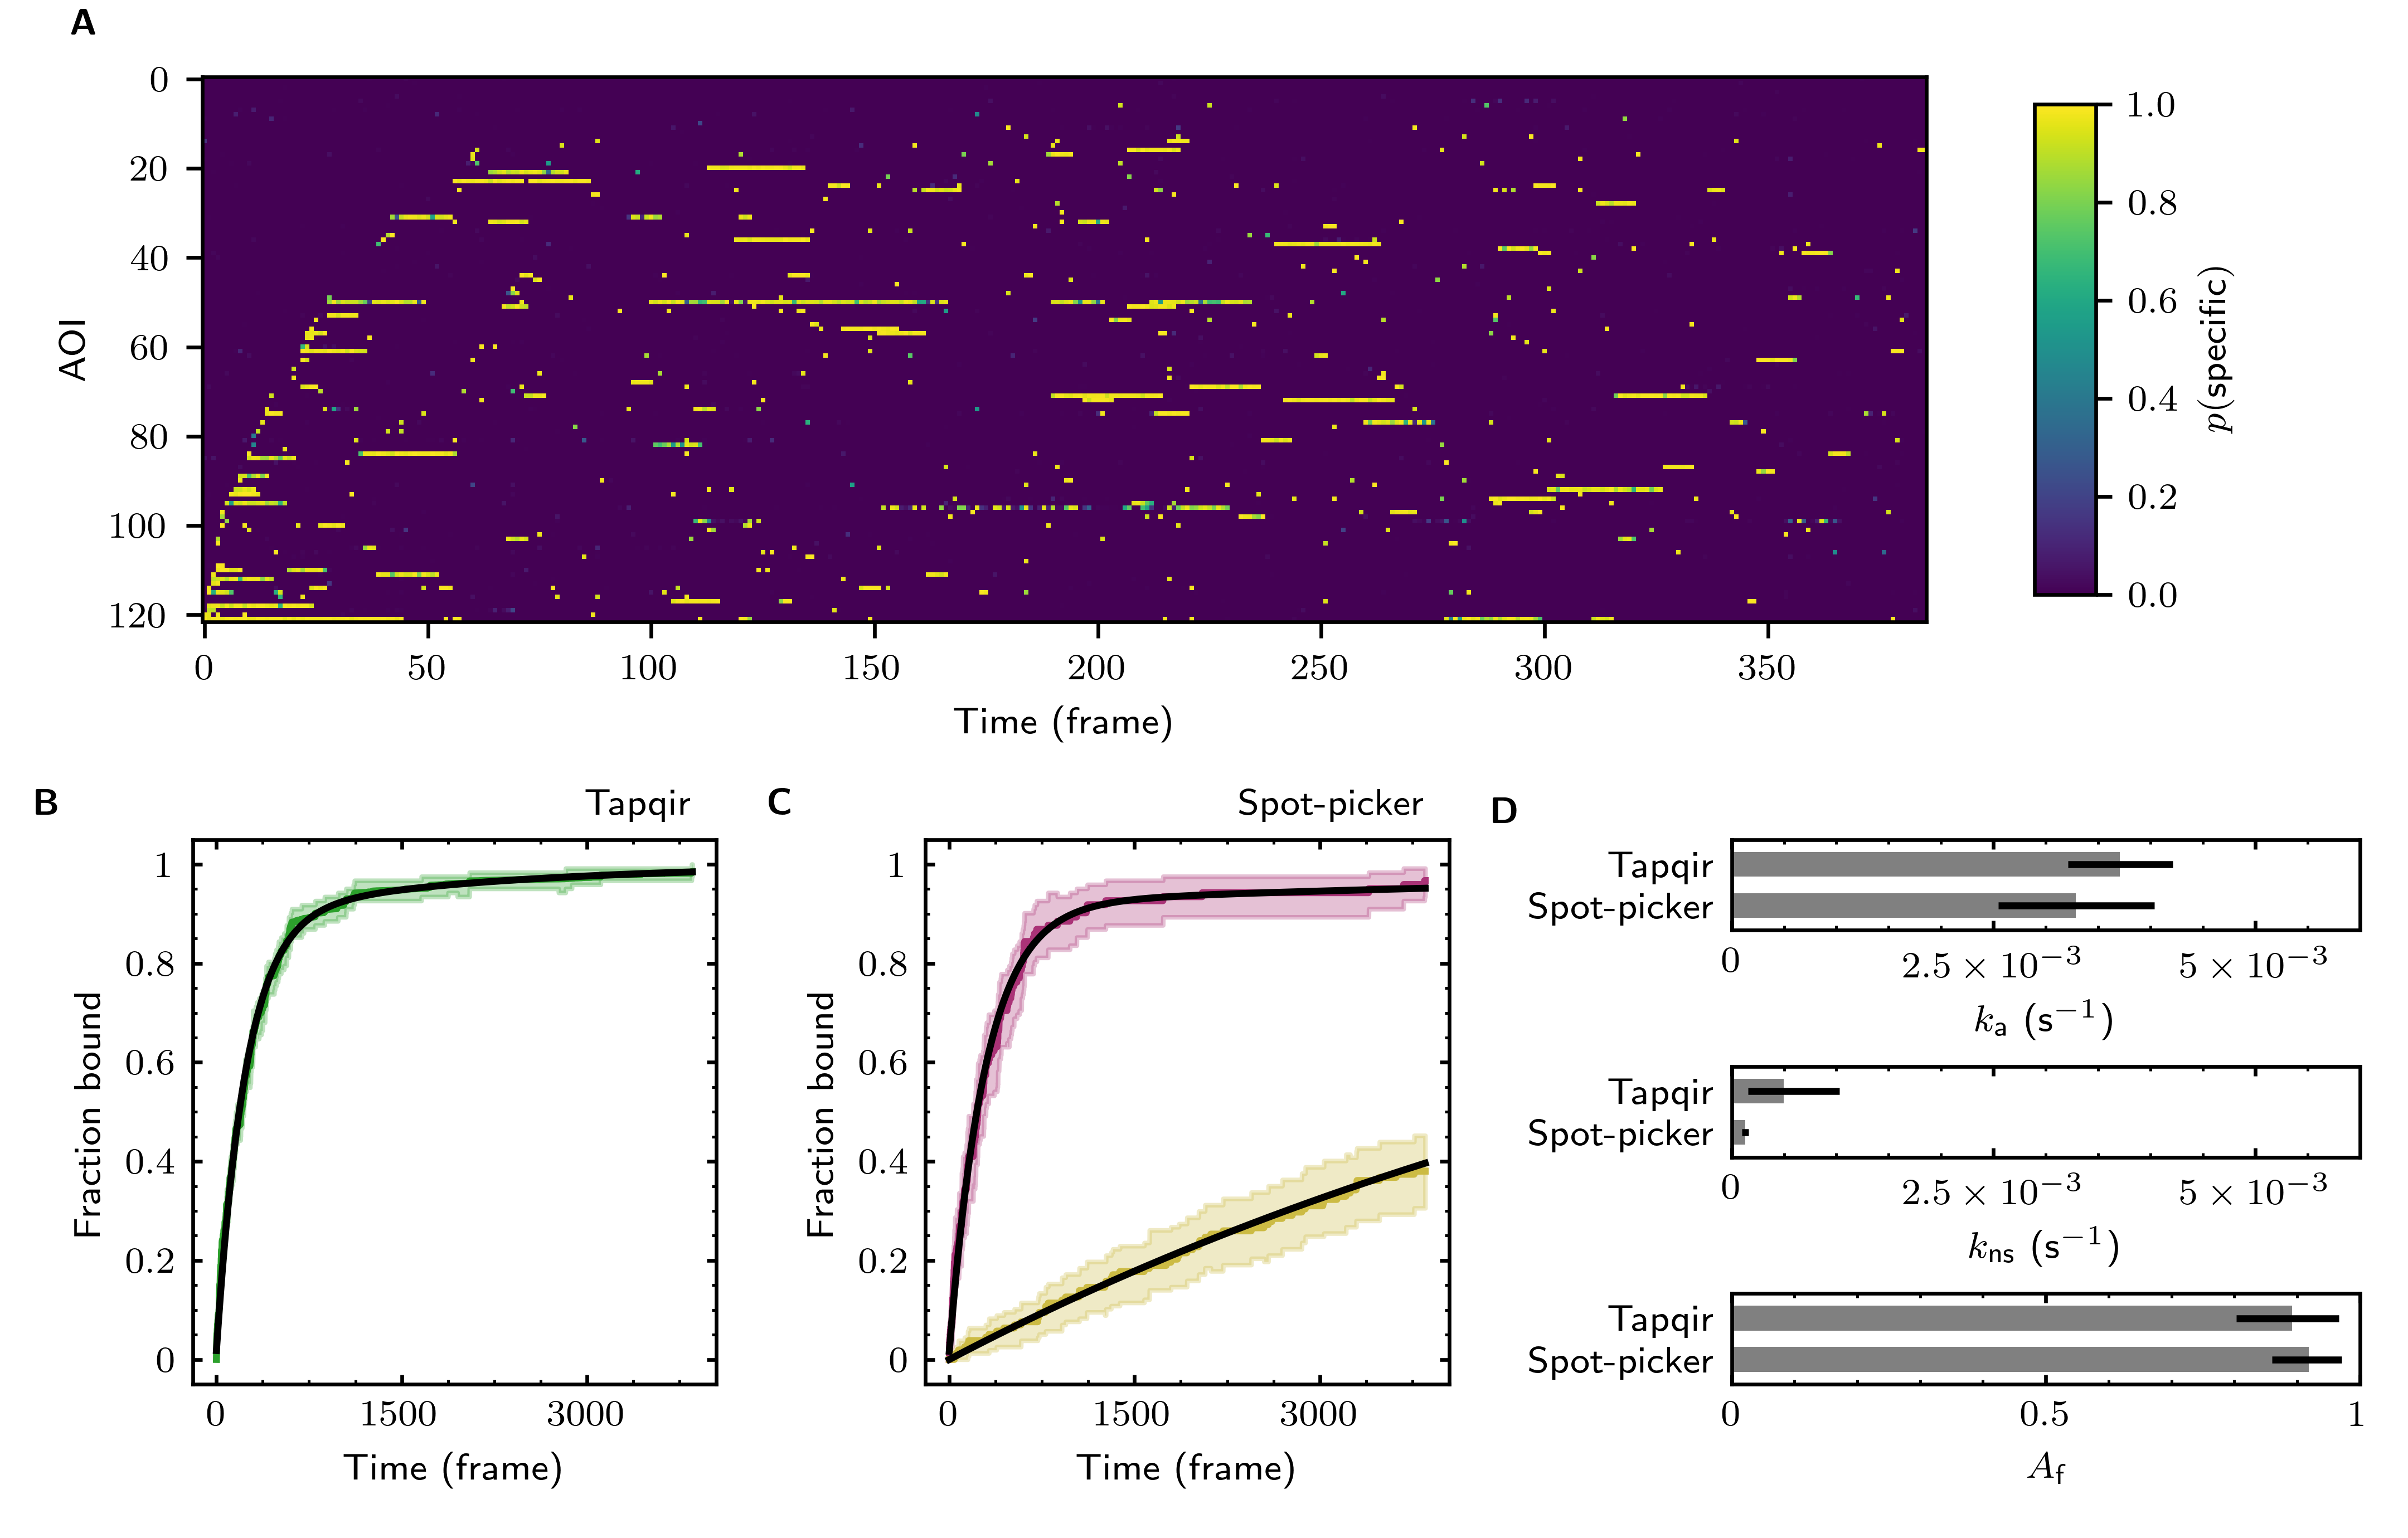
\includegraphics[width=183mm]{figures/experimental_data_DatasetC.png}}\label{figsupp:DatasetC}

\figsupp[Additional example showing extraction of target-binder association kinetics from experimental data.]{\textbf{Additional example showing extraction of target-binder association kinetics from experimental data.} Data are from Data set D ($\textrm{SNR} = 4.85$, $\lambda = 0.0404$; see \TABLE{datasets}).  Results are plotted as in \FIG{experimental_data}, except that for clarity only every $13^\mathrm{th}$ AOI is shown in (\textbf{A}).}{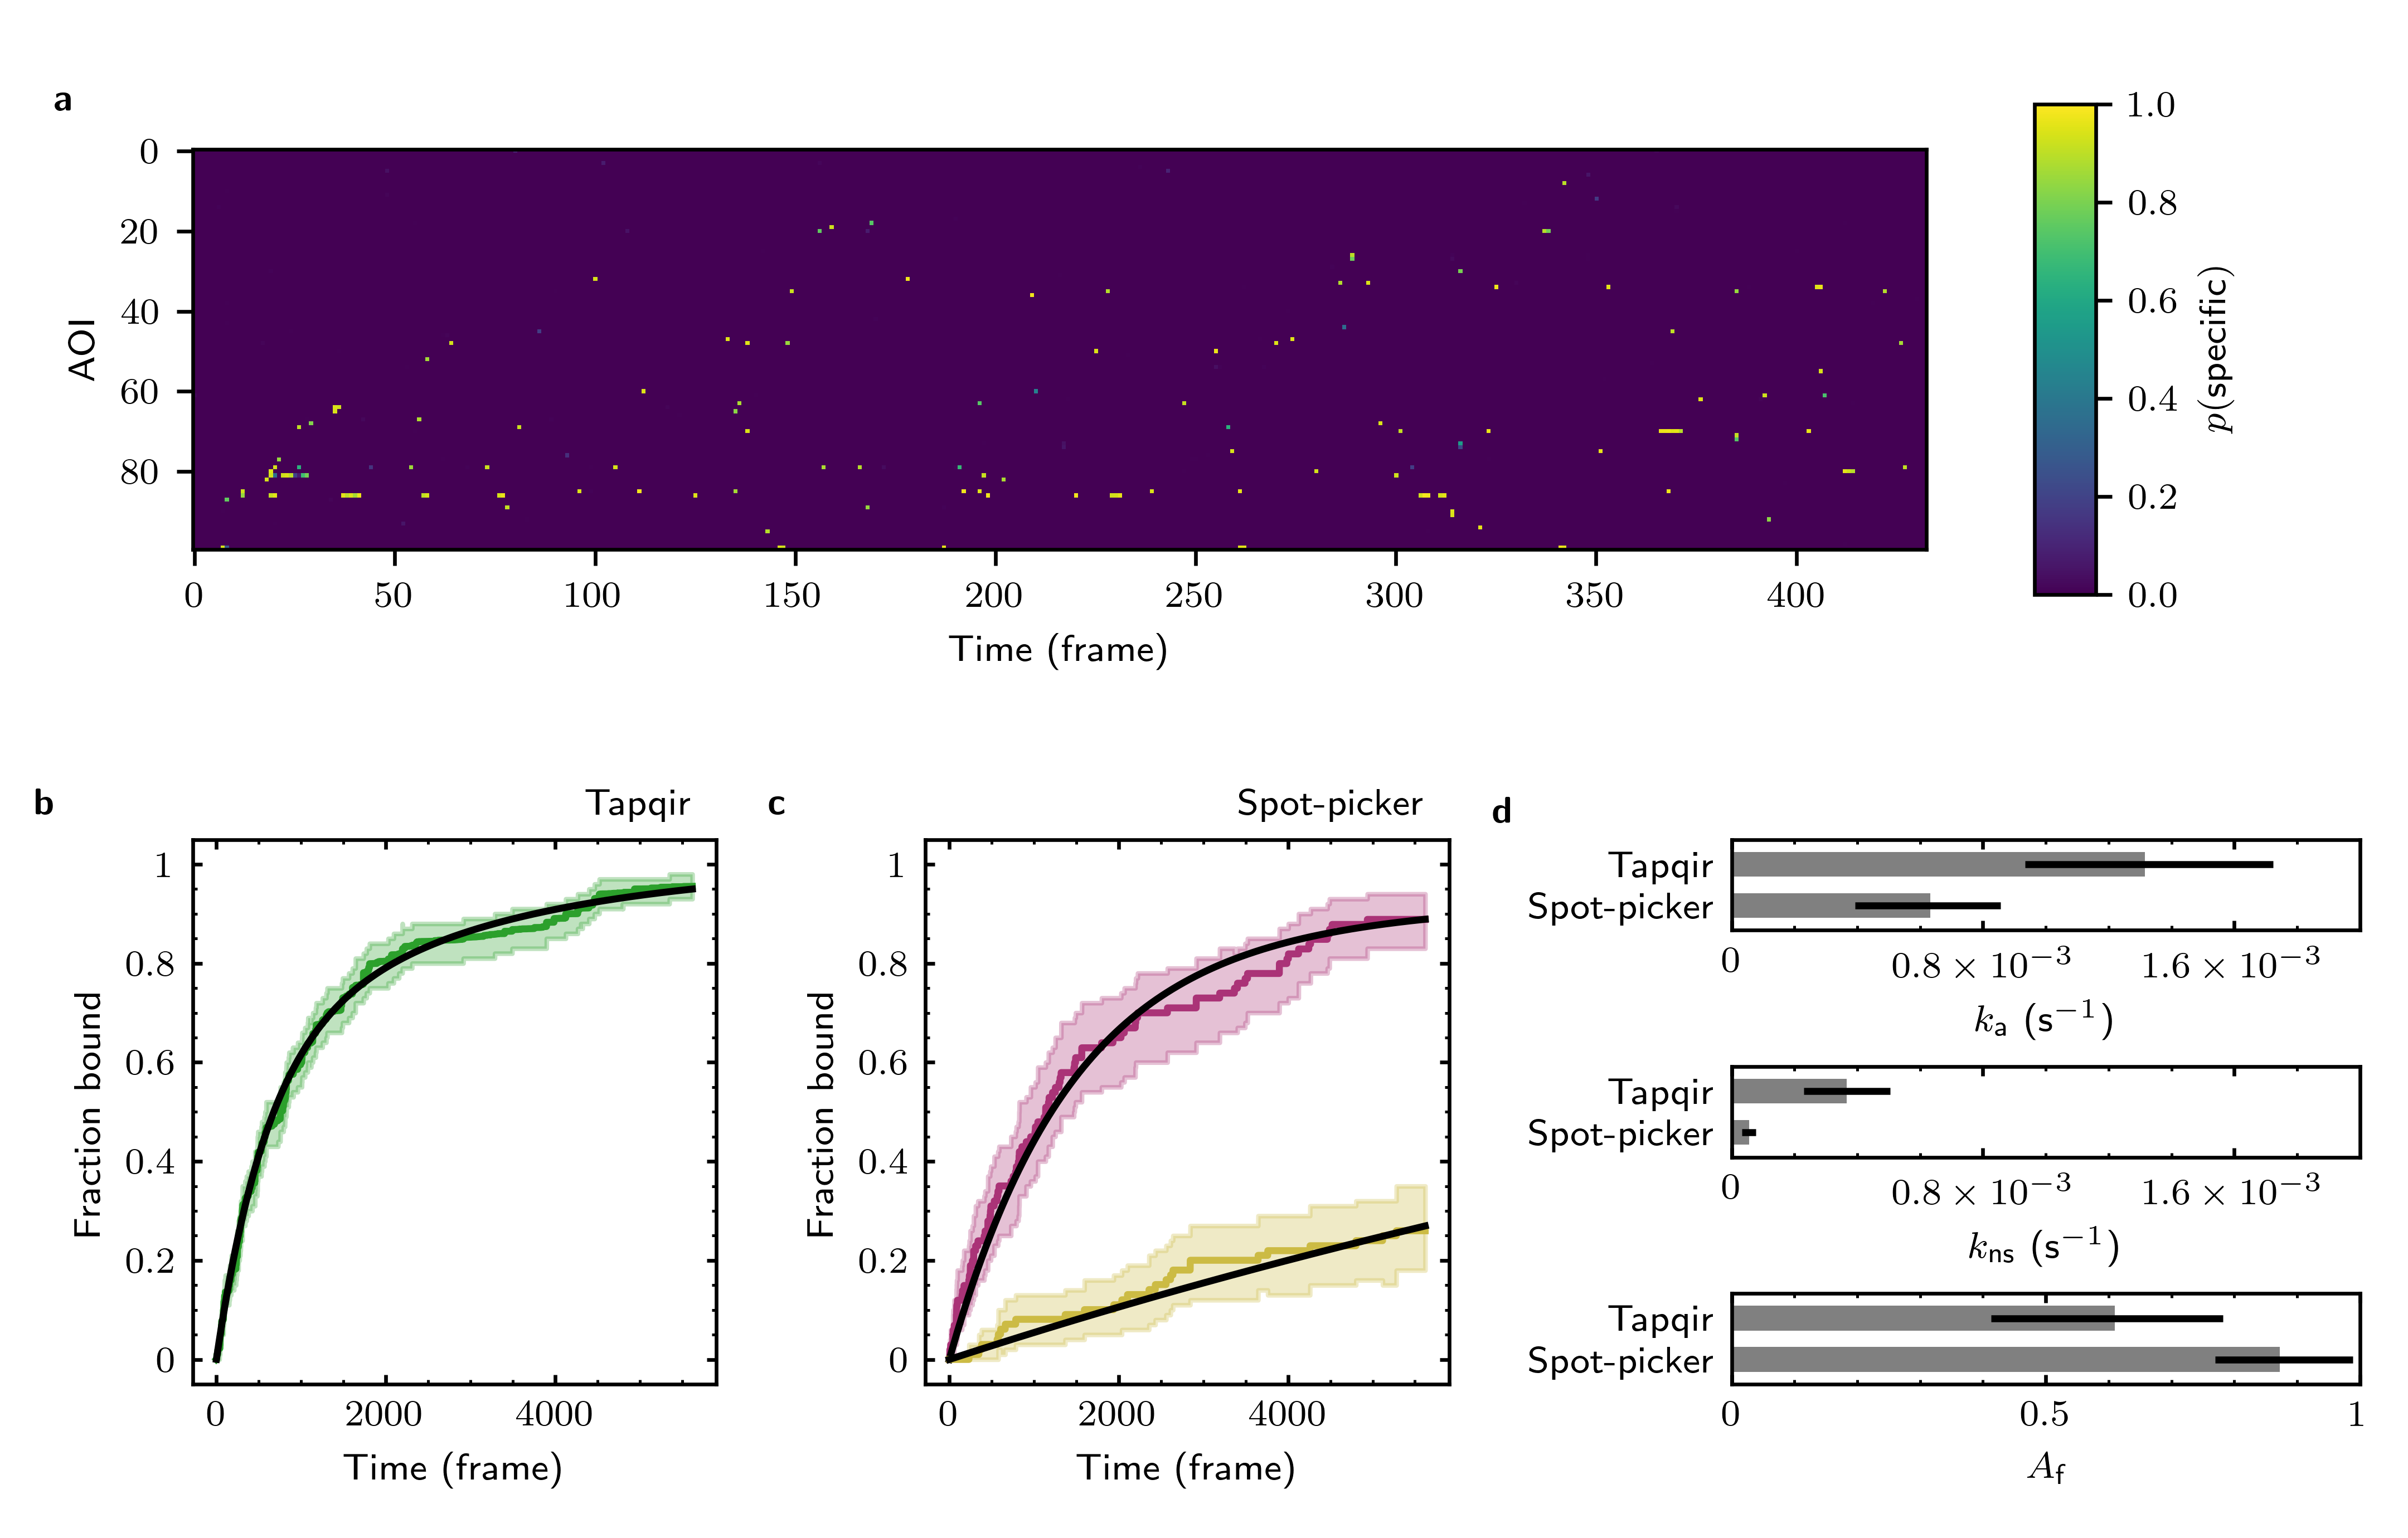
\includegraphics[width=183mm]{extended-data/figure8.png}}\label{figsupp:DatasetD}
\end{fullwidth}
\end{figure}

\begin{table}
\caption{\label{tab:datasets} \textbf{Experimental data sets.}}
\resizebox{\textwidth}{!}{%
% Use "S" column identifier to align on decimal point 
\begin{tabular}{ccccccc}
\toprule
Data set size\textsuperscript{a} & SNR & $\pi \: [95\% \: \mathrm{CI}]$ & $\lambda \: [95\% \: \mathrm{CI}]$ & $g \: [95\% \: \mathrm{CI}]$ & $\sigma^{xy} \: [95\% \: \mathrm{CI}]$ & Compute time\textsuperscript{b} \\
\midrule
\multicolumn{7}{l}{\parbox{1.4\textwidth}{Data set A: Binder, SNAP\textsubscript{f}-tagged \textit{S. cerevisiae} RNA polymerase II labeled with DY549; Target, transcription template DNA containing $5 \times$ Gal4 upstream activating sequences and \textit{CYC1} core promoter; Conditions, yeast nuclear extract supplemented with Gal4-VP16 activator and NTPs. From \cite{Rosen2020-zn}.}} \\
\\
\begin{tabular}[x]{@{}c@{}}$N = 331$, $N_\mathsf{c} = 526$\\$F = 790$\end{tabular} & $1.61$ &
$0.0951\:[0.0936, 0.0966]$ & $0.2943\:[0.2924, 0.2963]$ & $6.645\:[6.643, 6.647]$ & $0.577\:[0.573, 0.580]$ & 6 h \\
\midrule
\multicolumn{7}{l}{\parbox{1.4\textwidth}{Data set B: Binder, 0.1 nM \textit{E. coli} $\sigma^{54}$ RNA polymerase labeled with Cy3; Target, 852 bp DNA containing the \textit{glnALG} promoter; Conditions, physiological buffer, no NTPs. From  (Fig. 1E) of \cite{Friedman2013-sf}.}} \\
\\
\begin{tabular}[x]{@{}c@{}}$N = 102$, $N_\mathsf{c} = 127$\\$F = 4407$\end{tabular} & $3.77$ & $0.0846\:[0.0835, 0.0857]$ & $0.1575\:[0.1569, 0.1583]$ & $11.861\:[11.856, 11.865]$ & $0.476\:[0.474, 0.479]$ & 8 h 20 m \\
\midrule
\multicolumn{7}{l}{\parbox{1.4\textwidth}{Data set C: Binder, 0.4 nM \textit{E. coli} $\sigma^{54}$ RNA polymerase labeled with Cy3; Target,  3,591 bp DNA containing the \textit{glnALG} promoter; Conditions, physiological buffer, no NTPs. From (Fig. 3D) of \cite{Friedman2013-sf}.}} \\
\\
\begin{tabular}[x]{@{}c@{}}$N = 122$, $N_\mathsf{c} = 157$\\$F = 3855$\end{tabular} & $4.23$ & $0.0267\:[0.0262, 0.0273]$ & $0.0876\:[0.0869, 0.0883]$ & $16.777\:[16.773, 16.782]$ & $0.404\:[0.399, 0.408]$ & 5 h 45 m \\
\midrule
\multicolumn{7}{l}{\parbox{1.4\textwidth}{Data set D: Binder, 0.15 nM \textit{E. coli} Cy3-GreB; Target, reconstituted backtracked EC-6 \textit{E. coli} transcription elongation complex; Conditions, physiological buffer, no NTPs.  Randomly selected subset of data set from \cite{Tetone2017-za}.}} \\
\\
\begin{tabular}[x]{@{}c@{}}$N = 200$, $N_\mathsf{c} = 200$\\$F = 5622$\end{tabular} & $3.06$ & $0.0038\:[0.0036, 0.0039]$ & $0.0437\:[0.0434, 0.0440]$ & $18.727\:[18.724, 18.731]$ & $0.451\:[0.438, 0.463]$ & 6h \\
\bottomrule
\multicolumn{7}{l}{\footnotesize{\parbox{1.4\textwidth}{\textsuperscript{a}$N$ - number of on-target AOIs, $N_\mathsf{c}$ - number of control off-target AOIs, $F$ - number of frames.

\textsuperscript{b}Unattended calculation time on an AMD Ryzen Threadripper 2990WX with an Nvidia GeForce RTX 2080Ti GPU using CUDA version 11.4.}}} \rule{0pt}{3ex} \\
\end{tabular}}
\end{table}

\begin{table}[]
\caption{\label{tab:aoisize} \textbf{The effect of AOI size on classification accuracy.}\textsuperscript{a}}
\begin{tabular}{cccc}
    \toprule
    AOI dimension, $P$ (pixels) & MCC & Compute time\textsuperscript{b} \\
    \midrule
    $14$ & $0.951$ & 2 h 10 m \\
    $10$ & $0.948$ & 1 h 25 m \\
    $6$ & $0.939$ & 1 h 20 m \\
    \bottomrule
    \multicolumn{4}{l}{\footnotesize{\parbox{0.6\textwidth}{\rule{0pt}{3ex}\textsuperscript{a}Tapqir was applied to the same simulated data set (\texttt{height1000} parameter set in Supplementary File 3; SNR = 1.25) using different AOI sizes.
    
    \textsuperscript{b}Unattended calculation time on an AMD Ryzen Threadripper 2990WX with an Nvidia GeForce RTX 2080Ti GPU using CUDA version 11.5.}}} \rule{0pt}{3ex} \\
    \bottomrule
\end{tabular}
\end{table}